\section{Starter}
\subsection{My starter does not double in size}

Some bakers call for the sourdough starter to
double in size before using it.
The idea is to use the sourdough starter at
peak performance to ensure a
balanced fermentation in the main dough.

The doubling in size metric should be
taken with a grain of salt when judging
your starter. Depending on the flour
you use to feed the starter, different levels
of its rising can be expected.
For instance, if you use rye flour then only
very little gas from the
fermentation can be retained inside the
starter. In consequence, your
sourdough starter will not rise as much. It
could still be in healthy shape. If you use wheat flour with less gluten,
the starter will not rise as
much either. The reason is that you have a weaker
gluten network resulting in
more gas dispersing out of your dough.

That being said, it is recommended that you develop
your volume increase
metric. Your starter will increase in size and then
ultimately lose structure
and collapse. Observe the point before it collapses.
This is the point when
you should use your starter. This could be a
 \qty{50}{\percent} volume increase, 100
percent or \qty{200}{\percent}. It is always better to use
the starter a little bit
too early rather than too late. If you use the
starter later, reduce the
quantity that you use. If the recipe calls for a 20
percent starter quantity,
use only 10
percent starter in that case. Your starter will
regrow in your main dough.

On top of relying on the size increase, start
taking note of your starter's
smell. Over time you will be able to judge its
fermentation state based on the
smell. The stronger the smell becomes, the further
your dough has fermented.
This is a sign that you should use less starter
when making the actual dough.

Please refer to
Section~\ref{section:readying-starter}~``\nameref{section:readying-starter}''
for more information on the topic.



\subsection{What's the best starter feeding ratio?}

The best starter feeding ratio is commonly either 1:5:5 or 1:10:10.
In the case of 1:5:5 that's 1 part old starter,
5 parts flour and 5 parts water. If you are using a stiff starter,
use half the amount of water. So that's 1:5:2.5. Depending on when
you last fed your starter 1:10:10 might make more sense. If the starter
is old and hasn't been fed recently the 1:10:10 ratio is a better choice.
By reducing the starter inoculation ratio, you provide the microorganisms
with a cleaner environment. This way they can reproduce and regrow
into a more desirable balance to begin your dough fermentation.

Generally, think of your sourdough starter as a dough. Use the same
ratios you use for your bread dough for your starter. Your starter
should be trained in the same environment that you later use
for your dough. This way your starter is perfectly suited to
ferment the dough into which it is later inoculated.

The only exception to the 1:5:5 and 1:10:10 rule is the initial
starter set-up stage. For the first days during the starter-making
process there aren't enough microbes yet. So using a 1:1:1 ratio
can speed up the process. 
\subsection{What's the benefit of using a stiff sourdough starter?}

A regular sourdough starter has equal parts of
flour and water (\qty{100}{\percent} hydration). A stiffer
sourdough starter features a hydration level of 50 to \qty{60}{\percent}.

The stiff sourdough starter boosts the yeast part
of your starter more. This way your gluten degrades
slower and you can ferment for a longer period. This
is especially handy when baking with lower gluten flours.

You can read more about the topic of stiff sourdough
starters in Section~\ref{section:stiff-starter}.

\subsection{What's the benefit of using a liquid sourdough starter?}

The liquid starter will boost anaerobic bacterial
fermentation in your starter. This way your starter
tends to produce more lactic acid rather than acetic
acid. Lactic acid is perceived as milder and more
yogurty. Acetic acid can sometimes taste quite
pungent. Acetic acid can be perfect when making 
dark rye bread but not so much when making a fluffy
ciabatta-style loaf.

When converting your starter to a liquid starter you are
permanently altering the microbiome of your starter.
You cannot go back once you have eliminated acetic
acid-producing bacteria. So it is recommended to keep
a backup of your original starter.

A downside to the liquid starter is the overall
enhanced bacterial activity. This means the baked bread
will have more acidity (but milder). The dough will degrade
faster during fermentation. For this reason, you
will need to use strong high-gluten flour when using
this type of starter.

You can read more about the liquid starter in
Section~\ref{section:liquid-starter}

\subsection{My new starter doesn't rise at all}

Make sure that you use unchlorinated water.
In many areas of the world, tap water has
chlorine added to kill microorganisms. If that's
the case in your region, bottled spring water will
help.
You can also use a water filter with activated charcoal
which will remove the chlorine.
Alternatively, if you draw tap water into a pitcher or other
container and let it sit, loosely covered, the chlorine
should dissipate within 12--24~hours, and you have
the added advantage of automatically having
room-temperature water.

Make sure to use whole grain flour (whole wheat, whole rye, etc.).
These flours have more natural wild yeast and
bacterial contamination. Making a starter
from just white flour sometimes doesn't work.
Try to use organic unbleached flour to make
the starter. Industrial flour can sometimes
be treated with fungicides.

\subsection{I~made a starter, it rose on day 3 and now not anymore}

This is normal. As your starter is maturing, different
microorganisms are activated. Especially during
the first days of the process, bad microbes
like mold can be activated. These cause your
starter to rise a lot. With each subsequent
starter-feeding, you select the microbes that are best
at fermenting flour. For this reason, it is
recommended to discard the leftover unused starter
from the first days of the process. Later on, unneeded
starter amounts should never be thrown away. You can make
great discard bread out of it.

So just keep going and don't give up. The first big
rise is an indicator that you are doing everything
right. Based on my experience, it takes around 7
days to grow a starter. As you feed your starter
more and more, it will become even better at fermenting
flour. The first bread might not go exactly as you
planned, but you will get there eventually. Each
feeding makes your starter stronger and stronger.

\subsection{Liquid on top of my starter}

Sometimes a liquid, in many cases black liquid, gathers on top
of your sourdough starter. The liquid might have a pungent
smell to it. Many people confuse this with mold. I~have seen
bakers recommending to discard the starter because of this liquid.
The liquid is commonly known as \emph{hooch}. After a while
of no activity the heavier flour separates from the water. The flour
will sit at the bottom of your jar and the liquid will stay on top.
The liquid turns darker because some particles of the flour weigh
less than the water and float on top. Furthermore dead microorganisms
float in this liquid. This liquid is not a bad thing; it's actively
protecting your sourdough starter from aerobic mold entering through
the top.

\begin{figure}[!htb]
\begin{center}
  \includegraphics[width=0.5\textwidth]{hooch}
  \caption[Hooch] {Hooch building on top of a sourdough
      starter~\cite{liquid+on+starter}.}%
  \label{fig:hooch}
\end{center}
\end{figure}

Simply stir your sourdough starter to homogenize the hooch back
into your starter. The hooch will disappear. Then use a little bit of
your sourdough starter to set up the starter for your next bread.
Once hooch appears, your starter has likely fermented for a long
period of time. It might be very sour. This state of starter
is excellent to make discard crackers or a discard bread. Don't throw
anything away. Your hooch is a sign that you have a long fermented
dough in front of you. Compare it to a 2 year ripened Parmigiano cheese.
The dough in front of you is full of delicious flavor.

\subsection{Fixing a moldy sourdough starter}

First of all, making a moldy sourdough starter is very difficult.
It's an indicator that something might be completely off in your starter.
Normally the symbiosis of yeast and bacteria does not allow external
pathogens such as mold to enter your sourdough starter.
The low pH created by the bacteria is a very hostile environment
that no other pathogens like. Generally everything below a pH
of 4.2 can be considered food safe~\cite{food+safe+ph}. This
is the concept of pickled foods. And your sourdough bread
is essentially pickled bread.

I~have seen this happening especially when the sourdough
starter is relatively young. Each flour naturally contains
mold spores. When beginning a sourdough starter, all
the microorganisms start to compete by metabolizing the
flour. Mold can sometimes win the race and outcompete
the natural wild yeast and bacteria. In that case simply
try cultivating your sourdough starter again. If mold reappears
again, it might be a very moldy batch of flour. Try a different
flour to begin your sourdough starter with.

Mature sourdough starters should not go moldy unless the conditions
of the starter change. I~have seen mold appearing when the starter is stored
in the fridge and the surface dried out. It also sometimes forms on the
edges of your starter's container, typically in areas where no active
starter microorganisms can reach. Simply try to extract an
area of your starter that has no mold. Feed it again with flour and
water. After a few feedings, your starter should be back to normal.
Take only a tiny bit of starter: \qtyrange{1}{2}{\gram} are enough. They already
contain millions of microorganisms.

Mold favors aerobic conditions. This means that air is required in order
for the mold fungus to grow. Another technique that has worked for me
was to convert my sourdough starter into a liquid starter. This successfully
shifted my starter from acetic acid production to lactic acid production.
Acetic acid, similarly to mold, requires oxygen to be produced. After
submerging the flour with water, over time the lactic acid bacteria
outcompeted the acetic acid bacteria. This is a similar concept to pickled
foods. By doing this you are essentially killing all live mold fungi. You
might only have some spores left. With each feeding the spores will become
fewer and fewer. Furthermore, it seems that lactic acid bacteria produce
metabolites that inhibit mold growth~\cite{mold+lactic+acid+bacteria}.

\begin{figure}[!htb]
  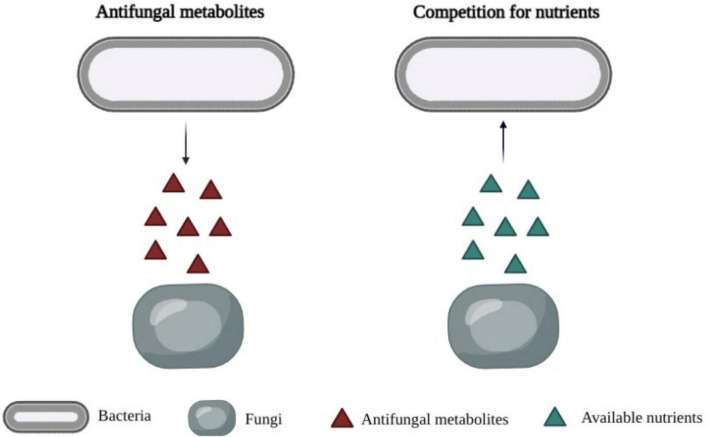
\includegraphics[width=\textwidth]{fungi-lactic-acid-interactions}
  \caption[The interaction of lactic acid bacteria and mold fungi]{The
      interaction of lactic acid bacteria and mold fungi.
      In~\cite{mold+lactic+acid+bacteria},
      \citeauthor{mold+lactic+acid+bacteria} et al.\ show how bacteria are
      producing metabolites that inhibit fungus growth.}%
  \label{fig:fungi-lactic-acid-interactions}
\end{figure}

To pickle your starter, simply take a bit of your existing starter (\qty{5}{\gram} for
instance). Then feed the mixture with \qty{20}{\gram} of flour and \qty{100}{\gram} of water. You have
created a starter with a hydration of around \qty{500}{\percent}. Shake the mixture vigorously.
After a few hours you should start seeing most of the flour near the bottom
of your container. After a while most of the oxygen from the bottom mixture
is depleted and anaerobic lactic acid bacteria will start to thrive. Take a
note of the smell your sourdough starter. If it was previously acetic
it will now change to be a lot more dairy. Extract a bit of your mixture the
next day by shaking everything first. Take \qty{5}{\gram} of the previous mixture, feed
again with another \qty{20}{\gram} of flour and another \qty{100}{\gram} of water. After 2--3
additional feedings your starter should have adapted. When switching back
to a hydration of \qty{100}{\percent} the mold should have been eliminated. Please note that
more tests should be conducted on this topic. It would be nice to really
carefully analyze the microorganisms before the pickling and after.

\subsection{My sourdough starter is too sour}

If your sourdough starter is too sour it will cause problems during
the fermentation. Your fermentation will have more
bacterial activity than yeast activity. This means
you will likely create a more tangy loaf which isn't
as fluffy as it could be. The goal is to reach the right
balance: Fluffy consistency from the yeast and a great,
not-too-strong tang from the bacteria. This depends
of course on what you are looking for in terms of taste
in your bread. When making rye bread, I~prefer to be more
on the tangy side for instance. When the described balance
is off, the first thing to check is your sourdough starter.

Note the smell of your starter. Does it smell very sour?
Taste a bit of your starter too. How sour does it taste?
Over time, every starter becomes more and more sour the longer
you wait. But sometimes your starter becomes sour too fast.
In this case apply daily feedings to your starter. Reduce
the amount of old starter that you use to feed. A ratio
of 1:5:5 or 1:10:10 can do wonders. In this case you would
take 1 part of starter (\qty{10}{\gram}) and feed it with \qty{50}{\gram} of flour
and \qty{50}{\gram} of water. This way the microorganisms start
the fermentation in a greenfield environment. This is
similar to the \qty{10}{\percent} starter or  \qty{20}{\percent} starter
ratio that you use to make a dough. These days I~almost
never use a 1:1:1 ratio. This only makes sense when you
are initially creating your starter. You want a sour
environment so that your microorganisms outcompete
potential pathogens. The acidic environment is toxic
to most pathogens that you do not want in your starter.

Another approach that can help is to convert your
sourdough starter into a stiff starter as
described in Section~\ref{section:stiff-starter}.

\subsection{Why does my starter smell like vinegar or acetone?}

Your sourdough starter has likely produced a lot of acetic acid.
Acetic acid is essential when creating vinegar. Once no additional
food is left some of your starter's bacteria will consume ethanol
and convert it into acetic acid. Acetic acid has a very pungent smell.
When tasting acetic acid, the flavor of your bread is often perceived
as quite strong.

\begin{figure}[!htb]
\begin{center}
  \footnotesize
\schemestart
\chemfig{H-C(-[2]H)(-[6]H)-C(-[2]H)(-[6]H)-O(-[7]H)} \+
\chemfig{O_2} \arrow
\chemfig{H-C(-[2]H)(-[6]H)-C(=[1]O)-[7]O-H} \+
\chemfig{H_2O}
\schemestop

  \caption{Oxygen is required to create acetic acid~\cite{acetic+acid+production}.}%
  \label{fig:ethanol-oxidation}
\end{center}
\end{figure}

This is nothing bad. But if you would like to change
the flavor of your final bread, consider converting
your sourdough starter into a liquid starter. This will
help to prioritize lactic acid-producing bacteria.
Your flavor will change to dairy compared to vinegary.
You can't go back though. After the conversion your starter
will never go back to acetic acid production because you have
changed the tides towards primarily lactic acid fermentation.
I~like to have a separate rye starter. In my experiments
rye starters tend to feature many acetic acid bacteria.
This starter is excellent when you want to make a very hearty,
strong-tasting bread. A pure rye bread tastes excellent when
made with such a starter. The flavor when taking a bite
is incredible. It nicely plays with soups as well. Just take
a bit of this bread and dip it in your soup.

\section{Dough}
\subsection{Should I~autolyse my dough?}

In \qty{95}{\percent} of all cases, an autolysis
makes no sense. Instead I~recommend
that you conduct a fermentolysis. You
can read more about the autolysis process in
Section~\ref{section:autolysis} and
more about the topic of fermentolysis
in Section~\ref{section:fermentolysis}.

The fermentolysis combines all the benefits
of the autolysis while eliminating disadvantages
such as having to knead the dough multiple times.

The autolysis only makes sense when you might
bake a fast-fermenting yeast-based dough with a
high yeast inoculation rate. But even in that
case you could just lower the amount of yeast
to fermentolyse rather than autolyse.

\subsection{My dough sample (aliquot) doesn't rise. What's wrong?}

If you see that your dough rises in size but your aliquot doesn't, chances
are that both are fermenting at different speeds. This can often
happen when the temperature in your kitchen changes. The aliquot
is more susceptible to temperature changes than the main dough.
Because the sample is smaller in size, it will heat up or cool down
faster.

For this reason, you must use room-temperature water when
making your dough. By having the same temperature in both the sample
and your dough, you make sure that both ferment at the same rate.

If the temperature in your room changes significantly during the day, your
best option is to use a see-through container. Mark the container to properly
measure your dough's size increase.

Another option could be to use a more expensive pH meter to measure your
dough's acidity buildup. You can read more about different ways of managing
bulk fermentation in Section~\ref{section:bulk-fermentation}.

\subsection{What's a good level of water (hydration) to make a dough?}

Especially when starting to make bread, use lower amounts of water. This will
greatly simplify the whole process. I~recommend using a level of around 60
percent hydration. So for every \qty{100}{\gram} of flour use around \qty{60}{\gram} of water.
This ballpark figure will work for most flours. With this hydration, you can
make bread, buns, pizzas, and even baguettes out of the same dough.

With the lower hydration, dough handling becomes easier and you have more yeast
fermentation, resulting in lower over-fermentation risk.

\subsection{My dough completely tears after a long fermentation}

Sometimes when touching your dough after a long fermentation
it completely tears apart. This could be for two reasons. It might
be that the bacteria completely consumed the gluten of your flour.
On the other hand, over time your gluten network automatically
degrades. This is the protease enzyme converting the gluten
network into smaller amino acids the seedling can use as
building blocks for its growth. This process starts to happen
the moment you mix flour and water. The longer your dough sits,
the more gluten is broken down. As the gluten holds the
wheat dough together, your dough will ultimately tear.

\begin{figure}[!htb]
  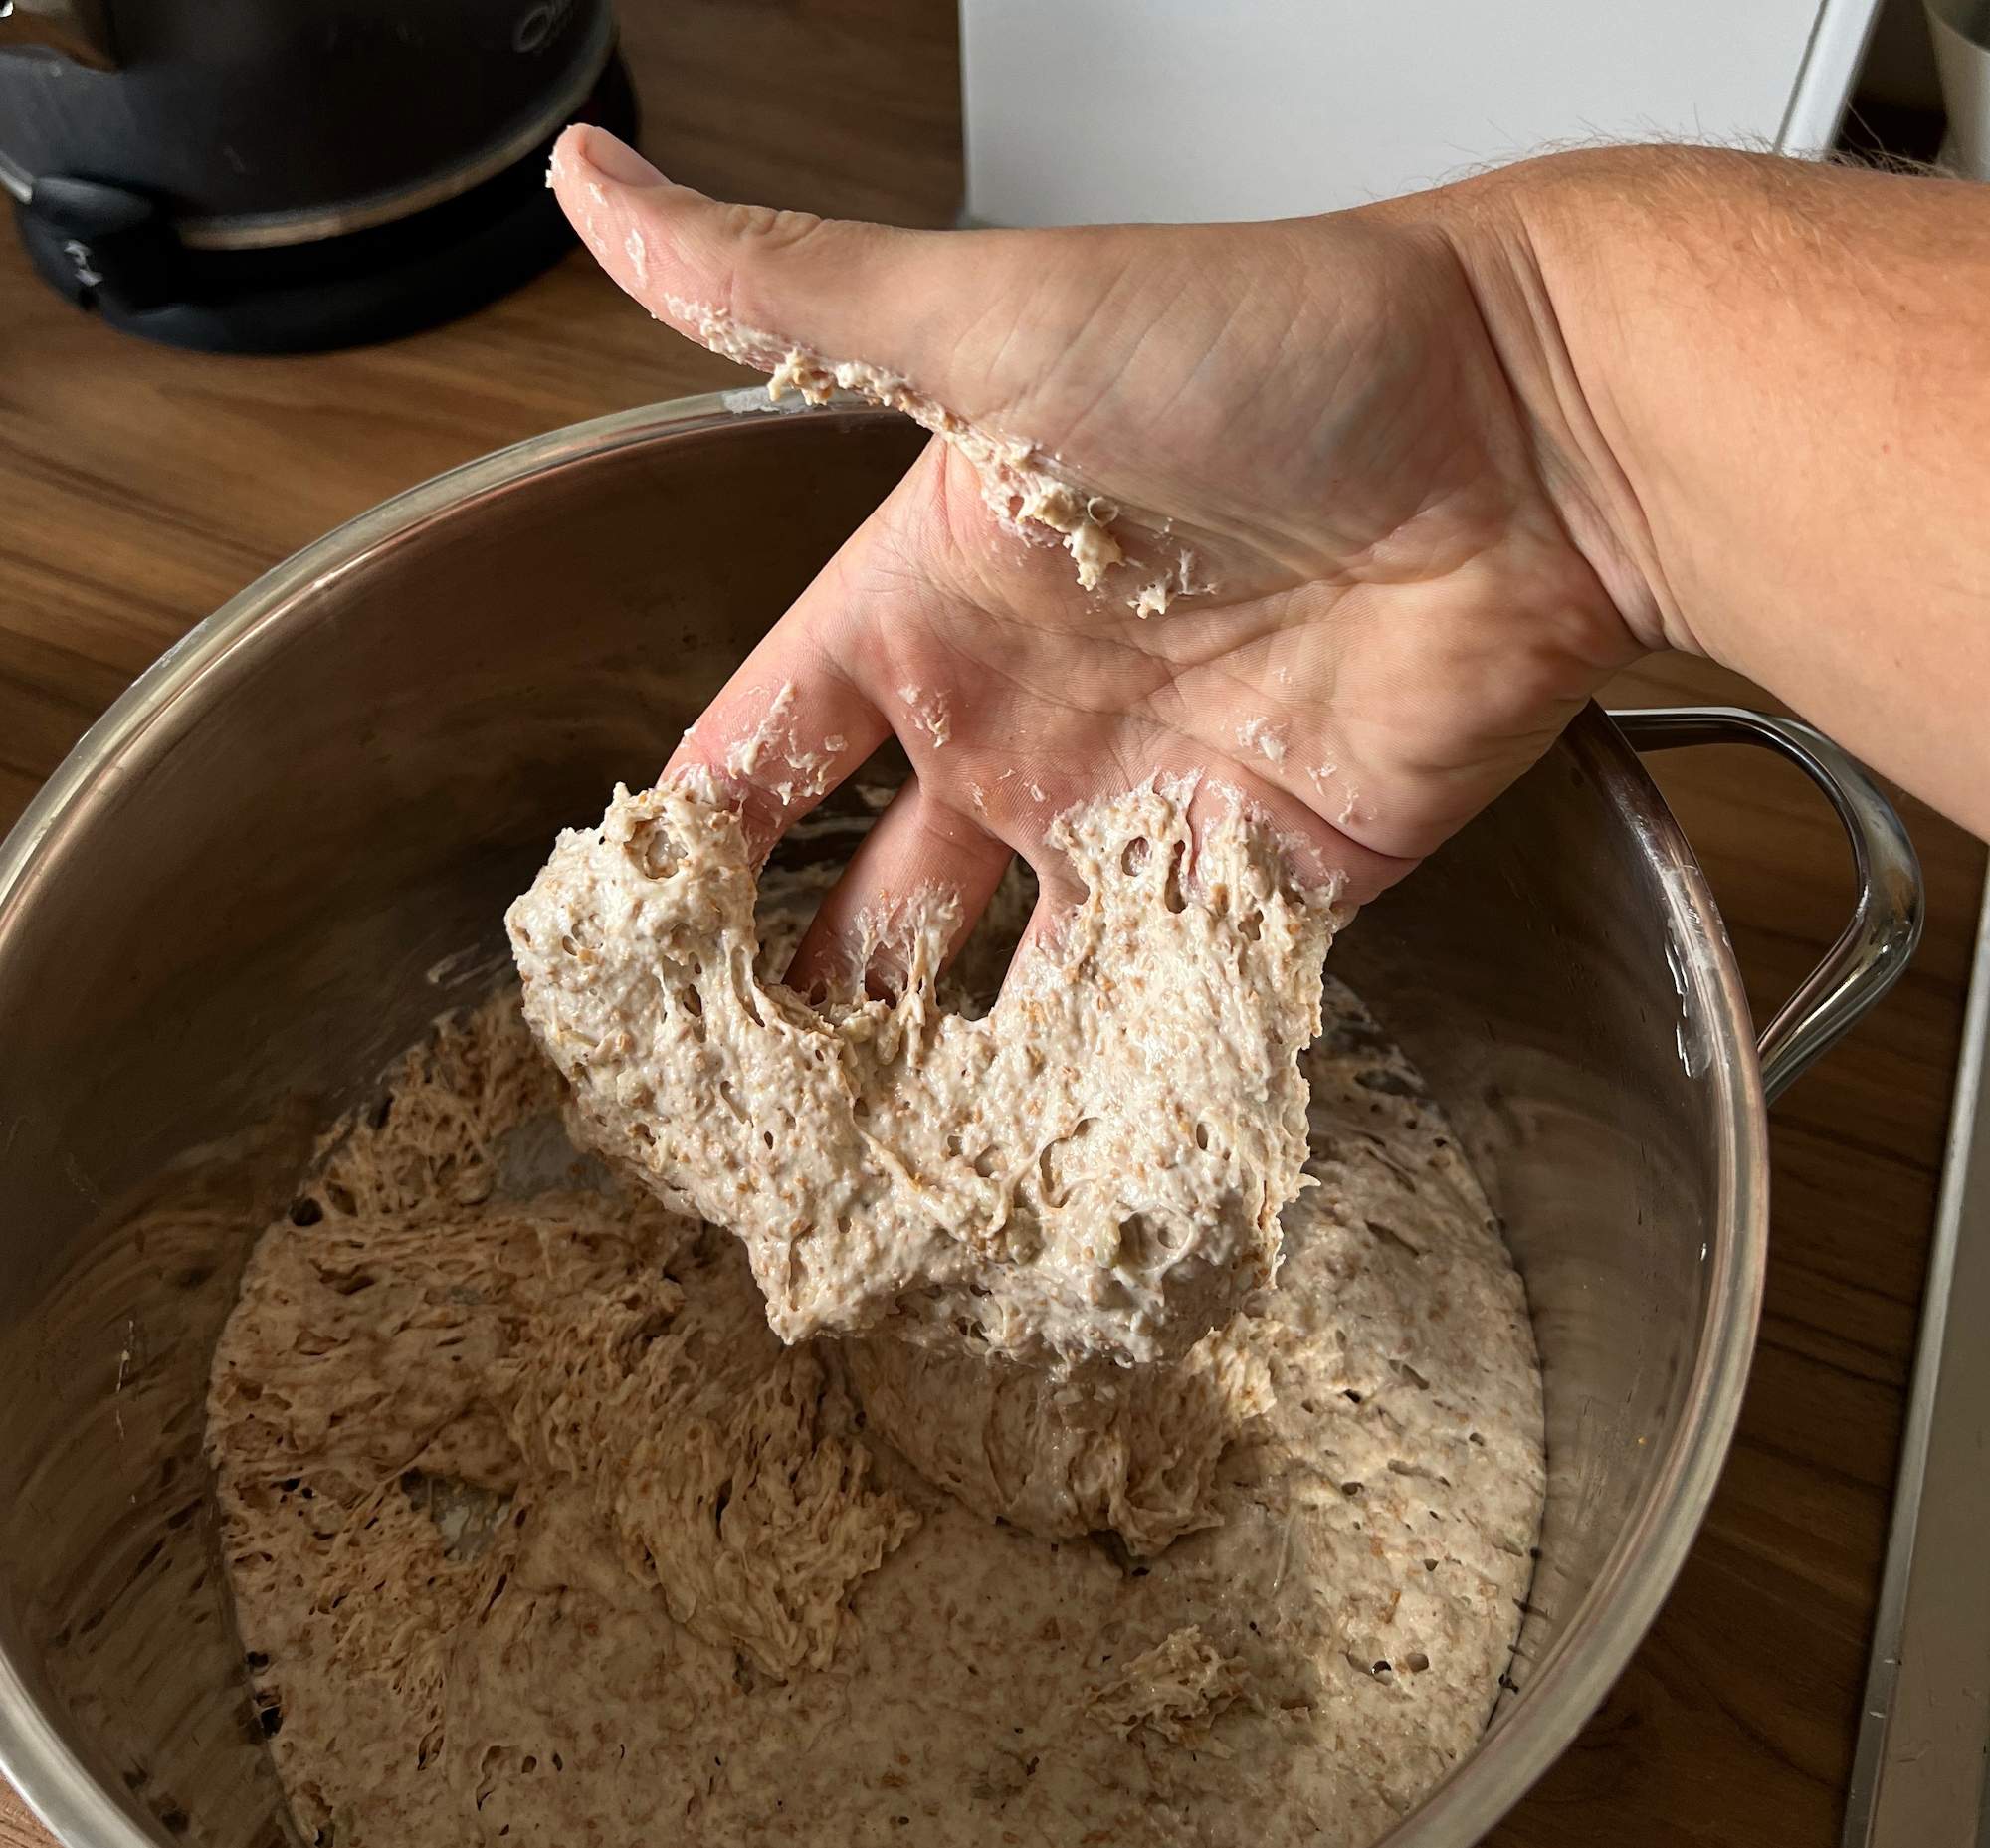
\includegraphics[width=1.0\textwidth]{tearing-dough}
  \caption[Dough tearing]{My dough tearing after 24~hours of no activity.}%
  \label{fig:tearing-dough}
\end{figure}

In the picture~\ref{fig:tearing-dough} I~experimented with
using a starter that has not been fed for 30 days at room temperature.
I~tried to make a dough directly out of the unfed starter.
Typically after a long period
without feedings your microbes start to sporulate and go
into hibernation mode. This way they can survive for a long
period of time without extra feedings. Adding additional food
will activate them again. In this case the dough did not ferment
fast enough before the protease broke down the gluten. By activating
your microbes they will start to reproduce and increase in quantity
for as long as there is food available. But this process
in my case was not fast enough. After around 24~hours, the whole
dough just started to completely tear apart. The whole process was further
accelerated by my using whole wheat flour. Whole wheat
contains more enzymes than white flour.

To fix this, try to make sure that your sourdough starter is lively
and active. Simply apply a couple more feedings before
making your dough. This way your dough becomes ready to shape
before it has completely broken down.

\section{Bread}
\subsection{My bread stays flat}

A flat bread is in most cases related to your gluten
network breaking down fully. This is not bad; this
means you are eating a fully fermented food. However,
from a taste and consistency perspective, it might be
that your bread tastes too sour, or is not fluffy anymore.
Please also note that you can only make bread with
great oven spring when making wheat based doughs. When
starting with this hobby I~always wondered why my rye
breads would turn out so flat. Yes, rye has gluten, but
small particles called \emph{hemicelluloses} (arabinoxylan and beta-glucan)~\cite{rye-defects}.
prevent the dough from developing a gluten network it can
with wheat. Your efforts will be in vain, and your dough will
stay flat. Only spelt- and wheat-based doughs have the capability
of retaining the \ch{CO2} created by the fermentation.

In most cases something is probably off with your
sourdough starter. This very often happens when the starter
is still relatively young and isn't as capable of
fermenting flour. Over time your sourdough
starter is going to become better and better.
Keep your sourdough starter at room temperature
and then apply daily feedings with a 1:5:5 ratio.
This would be 1 part old starter, 5 parts flour,
5 parts water. This allows you to achieve a better
balance of yeast and bacteria in your sourdough.
Even better could be the use of a stiff sourdough
starter. The stiff sourdough starter boosts
the yeast part of your starter. This allows you
to have less bacterial fermentation, resulting
in a stronger gluten network toward the end
of the fermentation~\cite{stiff+starter}. Please
also refer to the Subsection~\ref{subsec:overfermented-dough} where
I~explained more about overfermented doughs. You can also
refer to Section~\ref{section:stiff-starter} with more details on
making a stiff sourdough starter.

Furthermore, a stronger flour containing more gluten
will help you to push the fermentation further. This
is because your flour contains more gluten and will
take longer to be broken down by your bacteria. Ultimately,
if fermented for too long, your dough is also going
to be broken down and will become sticky and flat.

To debug whether the excess bacterial fermentation is the issue,
simply taste your dough. Does it taste very sour? If yes,
that's a good indicator. When working the dough, does it
suddenly become very sticky after a few hours? That's a
another good indicator. Please also use your nose to note
the smell of the dough. It shouldn't be too pungent.

\subsection{I~want more tang in my bread}

To achieve more tang in your sourdough bread, you have
to ferment your dough for a longer period of time.
Over time the bacteria will metabolize most of the
ethanol created by the yeast in your dough. The bacteria
mostly produce lactic and acetic acid. Lactic acid
is chemically more acidic than acetic acid but sometimes
not perceived as sour. In most cases a longer fermentation
is what you want. You will either need to utilize a loaf
pan to make your dough or use a flour that can withstand
a long fermentation period. A flour like this is typically
called a \emph{strong flour}. Stronger flours tend
to be from wheat varieties that have be grown in more
sunny conditions. Because of that, stronger flours tend
to be more expensive. For freestanding loaves, I~recommend
using a flour that contains at least \qty{12}{\percent} protein.
Generally, the more protein, the longer you can ferment your dough.

Another option to achieve a more sour flavor could be to
use a starter that produces more acetic acid. Based on my own
experience, most of my pure rye starters produced stronger acetic
notes. Chemically, the acetic acid isn't as sour, but when tasting
it will seem more sour. Make sure to use a starter that is at
a hydration of around \qty{100}{\percent}. Acetic acid production
requires oxygen. A starter that is too liquid tends to favor lactic
acid production because the flour is submerged in water. By submerging
the dough very little oxygen can pass through the water to the fermenting flour.
Because of this, only very little acetic acid can be produced. Over
time the acetic acid-producing bacteria will perish from your starter.

\begin{figure}[!htb]
  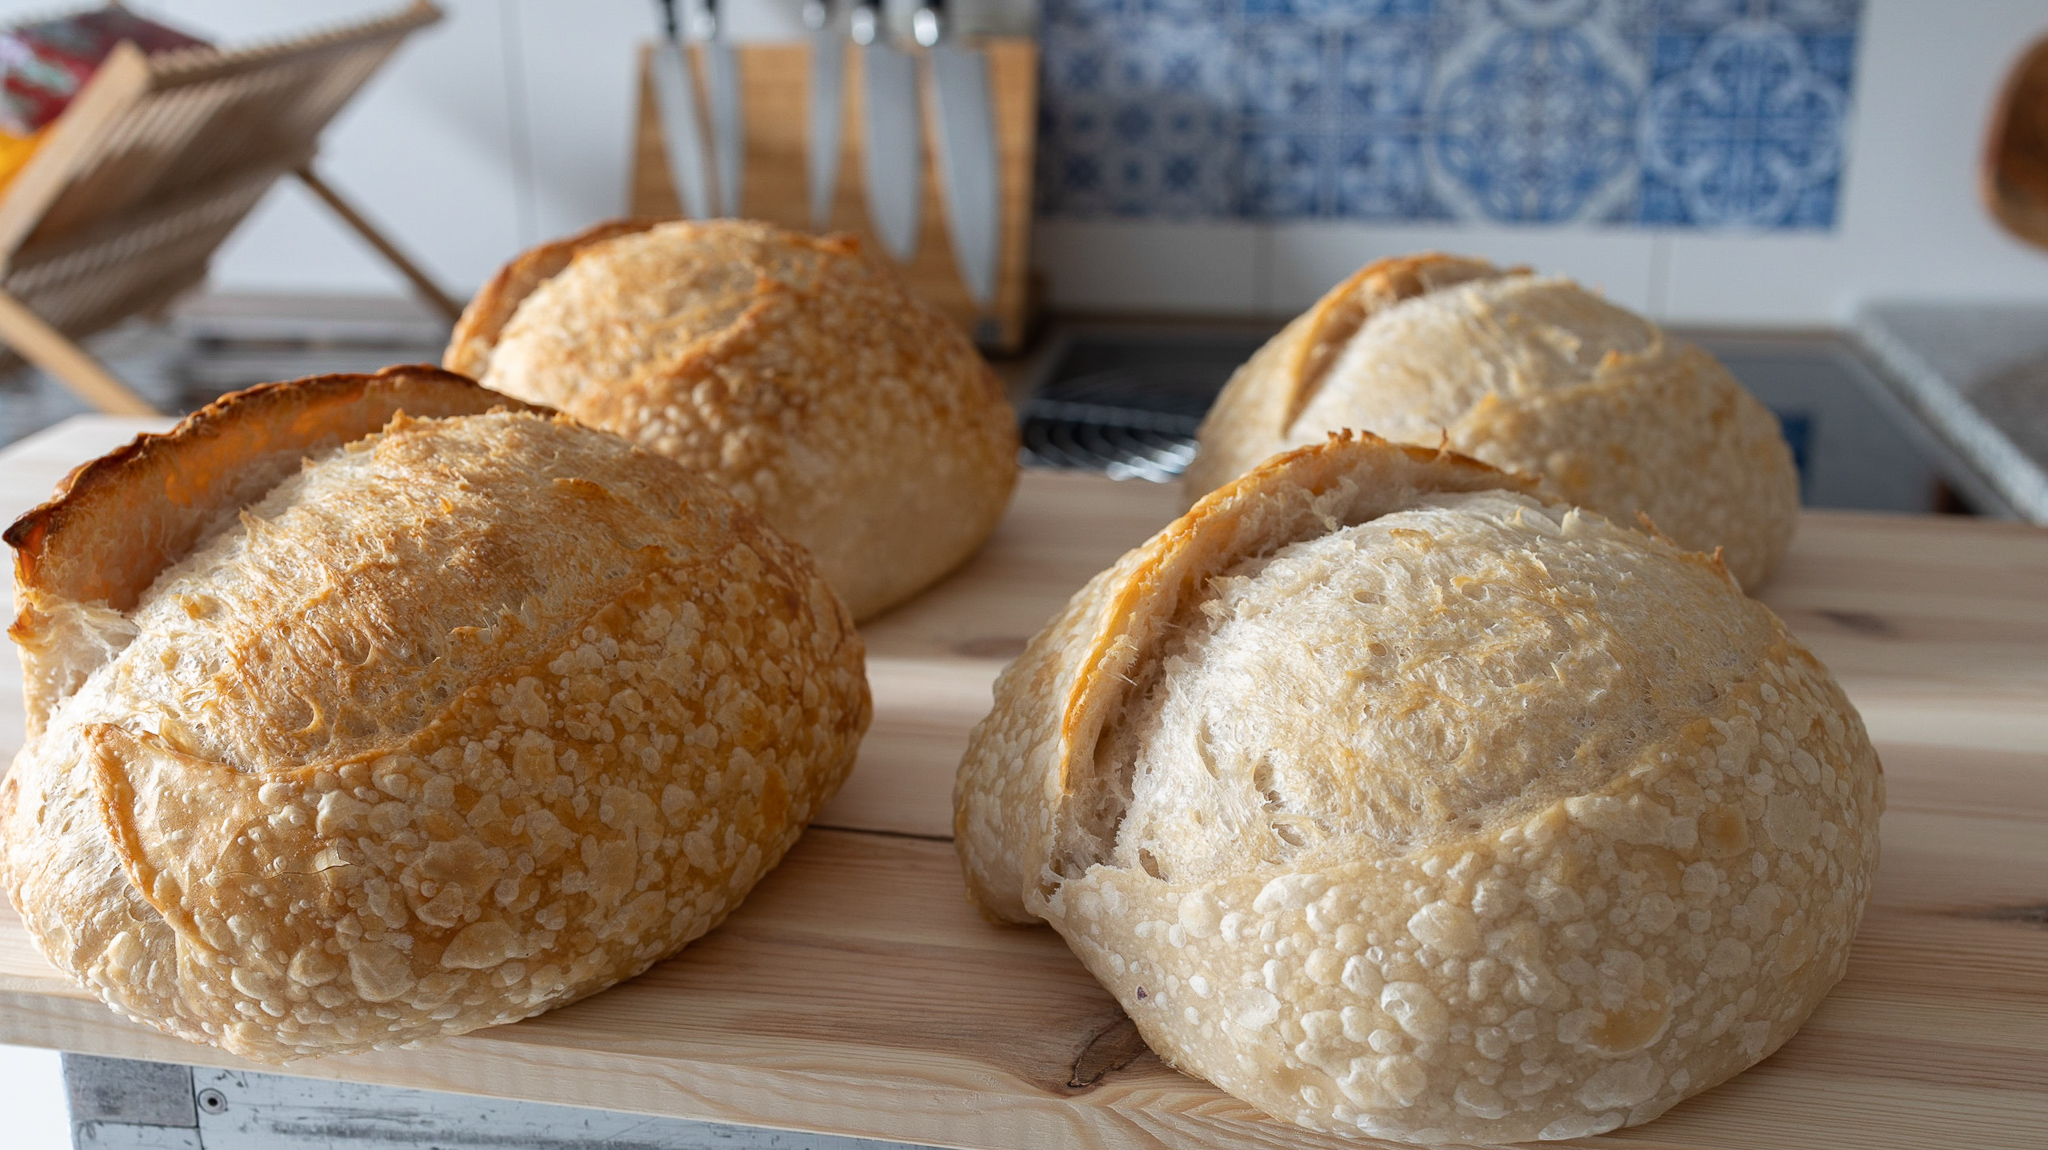
\includegraphics[width=\textwidth]{parbaked-bread.jpg}
  \caption[Half-baked bread]{A half-baked bread, known as \emph{parbaked}.}%
  \label{fig:parbaked-bread}
\end{figure}

Another easier option could be to bake your sourdough
twice. I~have observed this when shipping bread for my micro
bakery. The idea was to bake my bread for around 30~minutes
until it's sterilized, let it cool down and then ship it
to customers. Once you receive it, you just bake it again
for another 20--30~minutes to achieve the desired crust and
then you can eat it. Some of the customers reported a very sour
tasting bread. After investigating a bit more, it became
crystal clear. By baking the bread twice you don't boil off
as much acid during the baking process. Water
evaporates at around \qty{100}{\degreeCelsius} (\qty{212}{\degF}) while acetic
acid boils at \qty{118}{\degreeCelsius} (\qty{244}{\degF}) and lactic acid at
\qty{122}{\degreeCelsius} (\qty{252}{\degF}). After baking for 30~minutes at
around  \qty{230}{\degreeCelsius} (\qty{446}{\degF}) some of the water has
started to evaporate, but not all the acid yet. If you were to continue to
bake, more and more of the acid would start to evaporate. Now if you were to
stop baking after 30~minutes, you would typically have reached a core
temperature of around \qty{95}{\degreeCelsius} (\qty{203}{\degF}).  Your dough
would need
to be cooled down again to room temperature. The crust would
still be quite pale. Then a couple of hours later, you start
to bake your dough again. Your crust would become nice and
dark featuring delicious aroma. The aroma is coming from the
Maillard reaction. However, the core of your dough still won't
exceed the \qty{118}{\degreeCelsius} required to boil the acid. Overall, your
bread will be more sour. The enhanced acidity also helps
to prevent pathogens from entering your bread. The bread
will be good for a longer period of time. That's why
the concept of a delivery bakery works well with tangy sourdough bread.
In my own experiments, the bread stayed good for up to a week
in a plastic bag. This is much longer than a yeast-based dough that might
mold after just a few days\footnote{Some of my first test customers however
reported that the bread was overly sour and not pleasant to eat at all.
When this happens to you, consider toasting the bread. Toasting
will boil off additional acidity.}.

\subsection{My bread is too sour}

Some people like the bread less sour as well. This
is personal preference. To achieve a less sour bread
you need to ferment for a shorter period of time.
The yeast produces \ch{CO2} and ethanol. Both yeast and
bacteria consume the sugars released by the amylase enzyme
in your dough. When the sugar is depleted, bacteria starts to
consume the leftover ethanol by the yeast. Over time more
and more acidity is created, making a more sour loaf.

Another angle at this would be to change the yeast/bacteria
ratio of your sourdough. You can start the fermentation with
more yeast and less bacteria. This way, for the same given
volume increase of your dough, you will have less acidity.
A really good trick is to make sure that you feed your starter
once per day at room temperature. This way you shift
the tides of your starter towards a better yeast fermentation~\cite*{more+active+starter}.

To shift the tides even further, a real game changer
for me has been to create a stiff sourdough starter. The
stiff sourdough starter is at a hydration of around \qty{50}{\percent}.
By doing so your sourdough starter will favor yeast
activity a lot more. Your doughs will be more fluffy and less
sour for a given volume increase. I~tested this
by putting balloons over different glass jars. I~used
the same amount of flour for each of the samples.
I~tested a regular starter, a liquid starter and a stiff
starter. The stiff starter by far created the most \ch{CO2}
compared to the other starters. As a consequence, the stiff
starter balloon was inflated the most~\cite{stiff+starter}. You can read more
about the topic of stiff starters in Section~\ref{section:stiff-starter}.

Another unconventional approach could be to add baking
powder to your dough. The baking powder neutralizes the
lactic acid and will make a much milder
dough~\cite{baking+powder+reduce-acidity}.

\subsection{My bread flattens out when removing it from the banneton}

After removing your dough from the banneton, your dough will always
flatten out a bit. That's because over time your gluten network
relaxes and can no longer hold the shape. However, during the course
of baking, your dough is going to increase in size and inflate again.

If your dough however flattens out completely, it's a sign that
you have fermented your dough for too long. Please refer to
Subsection~\ref{subsec:overfermented-dough}
where I~explain about overfermented doughs. Your bacteria
has consumed most of your gluten network. That's why your
dough fully collapses and stays flat during the bake. The
\ch{CO2} and evaporating water will diffuse out of the dough.
A related symptom is that your dough sticks to the banneton.
When I~starting baking I~combated this with rice flour.
It worked for me but it might be a false find. Please refer to
Subsection~\ref{subsec:overfermented-dough} for more details on why
rice flour is not a good idea to manage sticky doughs.

These days I~gently rub my
dough with a bit of non-rice flour before placing it in
the banneton. Now if the dough starts to stick to the banneton
while I~remove it I~resort to a drastic measure. I~immediately
grease a loaf pan and directly place the dough inside. The loaf
pan provides a barrier and the dough can't flatten out as much.
The dough won't be as fluffy but it will be super delicious if you love tangy bread.

If you own a pH meter, take a note of your dough's pH before baking.
This will allow you to better judge your dough throughout
the fermentation process.

\subsection{My bread flattens out during shaping}

Similarly to a dough flattening out after removing it from the banneton,
a flattened dough after shaping is also a possible sign of over-fermentation.

When you try to shape the dough, can you easily tear pieces from the dough?
If yes, you have definitely overfermented your dough. If not, it might just
be a sign that you have not created enough dough strength for your dough.
A ciabatta, for instance, is a dough that tends to flatten out a bit after shaping.

If your dough is not able to be shaped at all, use a greased loaf pan
to rescue your dough. You can also cut a piece of the dough and use it
as the starter for your next dough. Your sourdough dough is essentially
just a gigantic starter.

\subsection{My crust becomes chewy}

Depending on which style of bread you are making a
thick crackly crust is sometimes desired. The crust
of your bread is created during the 2nd stage of the
baking process once the steaming source of your
oven has been removed. The dark colors are created by
the process known as \emph{Maillard reaction} and then followed
by another process known as \emph{caramelization}. Each
color of crust offers the taster a different aroma.

What happens quite often is that the crust becomes chewy after a day.
Sometimes when baking in the tropics with high humidity, the
crust only stays in this stage for a few hours. Afterwards
the crust becomes chewy. It's no longer as crisp compared
to the moment after baking. Your dough still contains moisture.
This moisture will start to homogenize in the final bread and
partially evaporate. The result is that your crust becomes chewy.

Similarly when storing your bread in a container or in a plastic
bag, your crust is going to become chewy. I~have no fix for this yet.
I~typically tend to store my breads in a plastic bag inside of my fridge.
This allows the moisture to stay inside of bread. When taking a slice
I~always toast each slice. This way some of the crispness returns.
If you know of a great way, please reach out and I~will update
this book with your findings.

\section{Debugging your crumb structure}%
\label{section:debugging-crumb-structure}

The crumb structure of your bread provides insights into how well
your fermentation process has gone. You can also spot common flaws
arising from improper technique. This chapter will provide you with information
that you can use to debug your baking process.

\begin{figure}
  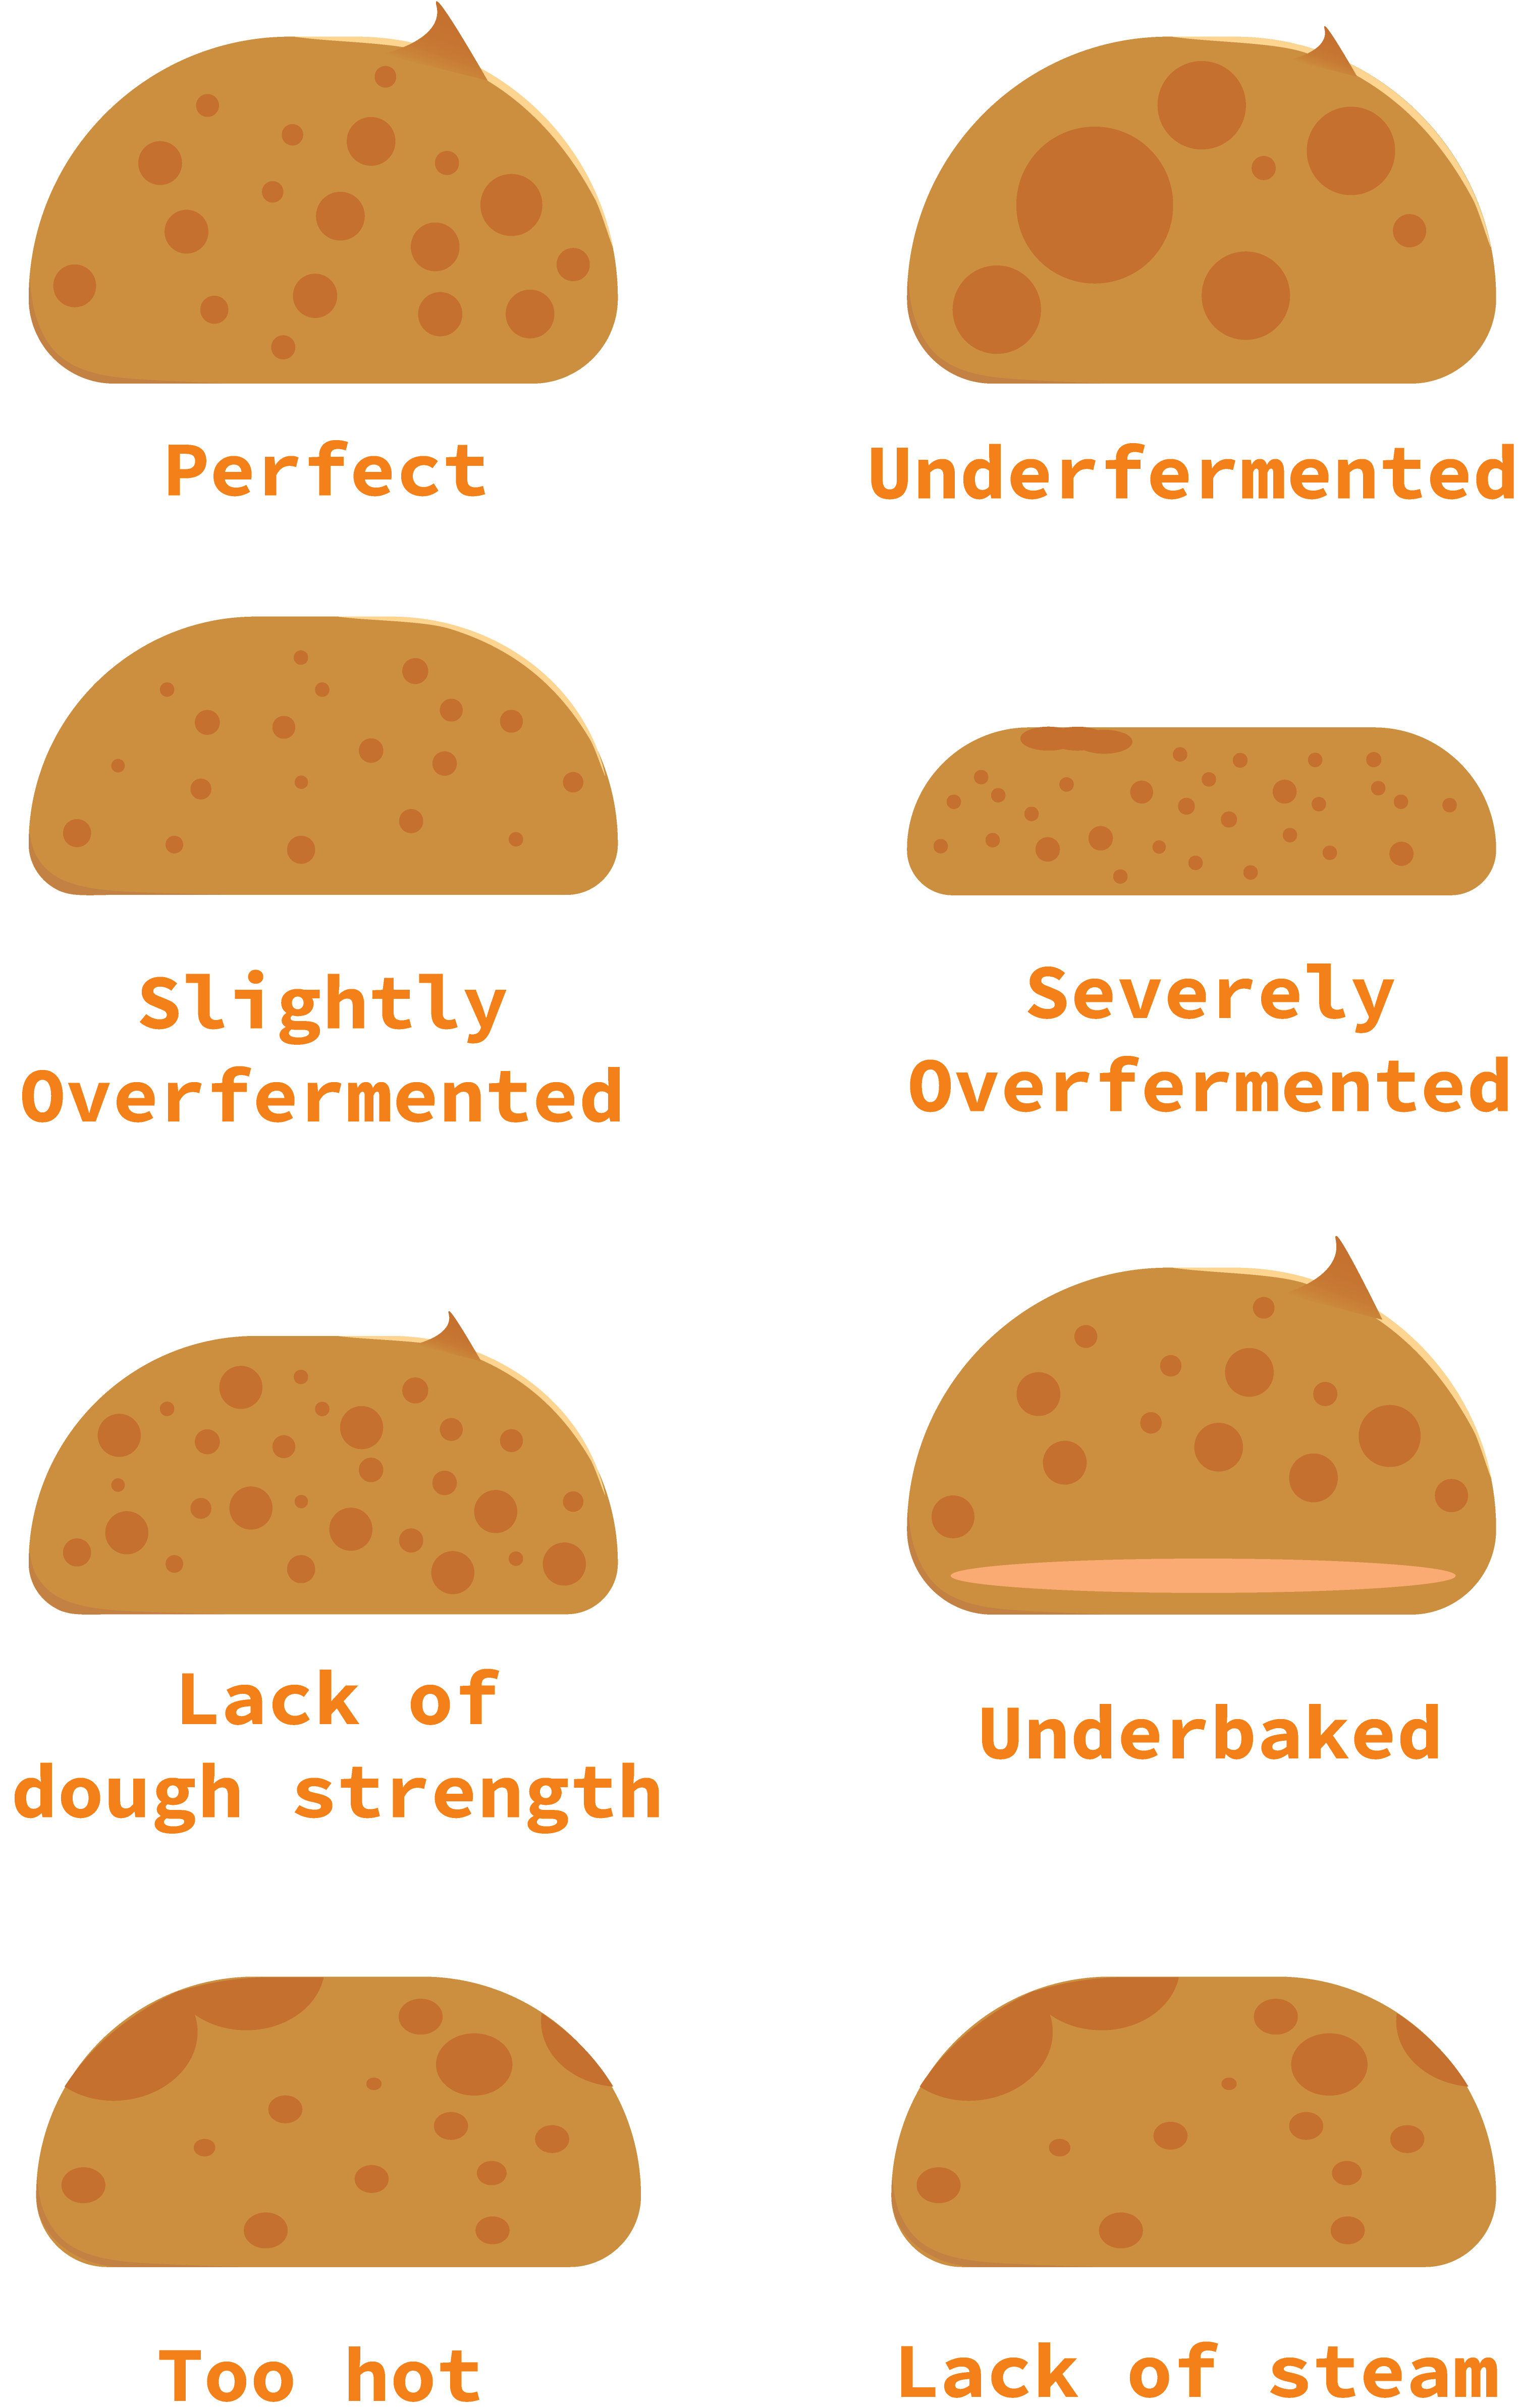
\includegraphics[width=\textwidth]{crumb-structures-book}
  \caption{A schematic visualization of different crumb structures and their respective causes. The
  final bread's crumb is a key aspect to identify potential issues related to fermentation
  or baking technique.}%
  \label{fig:crumb-structures-book}
\end{figure}

\subsection{Perfect fermentation}=

\begin{figure}
  \includegraphics[width=\textwidth]{open-crumb}
  \caption{The bread has a somewhat open crumb with areas
  featuring a honeycomb structure.}%
  \label{fig:open-crumb}
\end{figure}

Of course the perfect fermentation is debatable and highly subjective. To
me the perfect sourdough bread features a crisp crust paired with a fluffy,
somewhat open crumb. This is the perfect balance of different consistencies
when you take a bite.

Some people are chasers of a very open crumb, meaning you have large pockets
of air (alveoli). It's subjective whether that's the style of bread that you like;
however, to achieve it you need to ferment your bread dough perfectly.
It takes a lot of skill both in terms of mastering fermentation and technique
to achieve a crumb structure like that.

Personally, I~like a bread like that, just with a slightly less wild crumb.
The style of crumb I~like is called the \emph{honeycomb crumb}. It's not too open, but
just enough open to make the bread very fluffy. To achieve the previously mentioned open crumb, you
have to touch your dough as little as possible. The more you interact with your
dough, the more you are degassing your dough. Excess touching of the dough
results in the dough's alveoli merging together. The crumb will not be as open.
That's why achieving such a crumb works best if you only ferment
one loaf at a time. Normally, if you have to pre-shape your dough,
you will automatically degas your dough a little bit during the rounding process.
If you skip this step and directly shape your dough, you will achieve a more open crumb.
A good rule of thumb is to not touch your dough for at least 1--2 hours before shaping,
to achieve as open a crumb as possible.

\begin{figure}
  \includegraphics[width=\textwidth]{honeycomb}
  \caption{A whole wheat sourdough with an almost exclusive honeycomb crumb
  structure.}%
  \label{fig:honeycomb}
\end{figure}


Now this is problematic when you want to
make multiple loaves at the same time. Pre-shaping is essential as you are required
to divide your large bulk dough into smaller chunks. Without the pre-shaping
process, you would end up with many non-uniform bread doughs. This technique is
also used when making ciabattas. They are typically not shaped. You only cut the
bulk dough into smaller pieces, trying to work the dough as little as possible.
With pre-shaping you will converge your dough's alveoli into more of a honeycomb structure,
as large pockets of air will slightly merge. Similarly to the open crumb structure,
you also have to nail the fermentation process perfectly to achieve this crumb.
Too long a fermentation will result in gas leaking out of your dough while baking.
The honeycombs won't be able to retain the gas. If you ferment for too short a time,
there is not enough gas to inflate the structures. To me this is the perfect
style of crumb. As someone who appreciates jam, no jam will fall through a slice
of this bread compared to an open crumb.

\subsection{Overfermented}%
\label{sec:overfermented-dough}

\begin{figure}
  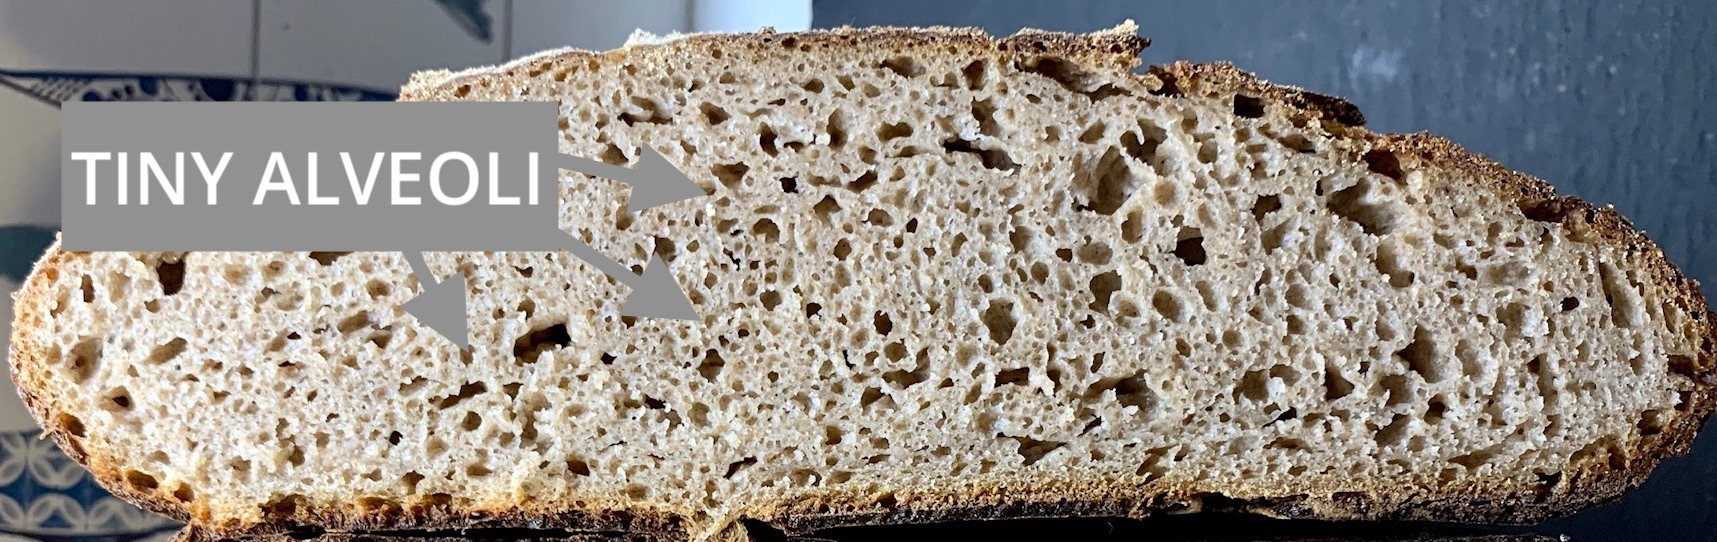
\includegraphics[width=\textwidth]{fermented-too-long}
  \caption{A relatively flat dough that has many tiny pockets of air.}%
  \label{fig:fermented-too-long}
\end{figure}

When fermenting your dough for too long, the protease enzyme starts to
break down the gluten of your flour. Furthermore, the bacteria consume the gluten
in a process called \emph{proteolysis}~\cite{raffaella+di+cagno}.
Bakers also refer to this process as \emph{gluten rot}.
The gluten that normally traps the \ch{CO2} created
by the fermentation process of your microorganisms can no longer keep the
gas inside of the dough. The gas disperses outward resulting in smaller alveoli in your crumb.
The bread itself tends to be very flat in the oven. Bakers often refer
to this style of bread as a \emph{pancake}. The oven spring can be compared
to bread doughs made out of low-gluten flour like einkorn.

Your bread will feature a lot of acidity, a really strong distinctive tang. From
a taste perspective, it might be a little bit too sour. From my own tests with family and
friends (n=15--20), I~can say that this style of bread is typically
appreciated less. However, I~personally really like the hearty strong taste.
It is excellent in combination with something
sweet or a soup.  From a consistency perspective, it is no longer as fluffy as it could be.
The crumb might also taste a little bit gummy. That's because it has been broken down a lot
by the bacteria. Furthermore, this style of bread has a significantly lower amount of gluten~\cite{raffaella+di+cagno}
and is no longer comparable to raw flour, it's a fully fermented product.
You can compare it with a blue cheese that is almost lactose free.

When trying to work with the dough, you will notice that suddenly the dough feels
very sticky. You can no longer properly shape and work the dough. When trying to
remove the dough from a banneton, the dough flattens out a lot. Furthermore,
in many cases your dough might stick to the banneton. When beginning with baking
I~would use a lot of rice flour in my banneton to dry out the surface of the dough a lot.
This way the dough wouldn't stick, despite being overfermented. However as it
turns out the stickiness issue has been my lack of understanding the fermentation
process. Now I~never use rice flour, except when trying to apply decorative scorings.
Properly managing fermentation results in a dough that is not sticky.

If you are noticing, during a stretch and fold or during shaping, that your dough
is suddenly overly sticky, then the best option is to use a loaf pan. Simply take
your dough and toss it into a loaf pan. Wait until the dough mixture has increased
in size a bit again and then bake it. You will have a very good-tasting sourdough
bread. If it's a bit too sour, you can just bake your dough for a longer period
of time to boil away some of the acidity during the baking process. You can also use
your dough to set up a new starter and try again tomorrow. Lastly, if you are hungry,
you can simply pour some of your dough directly into a heated pan with a bit of
oil. It will make delicious sourdough flatbreads.

To fix issues related to over-fermentation, you need to stop the fermentation process
earlier. What I~like to do is to extract a small fermentation sample from my dough.
Depending on the volume increase of this sample, I~can mostly judge when my fermentation
is finished. Try to start with a 25 percent volume increase of your main dough or sample.
Depending on how much gluten your flour has, you can ferment for a longer period of time.
With a strong flour featuring a 14--15 percent protein, you should be able to safely
ferment until a 100 percent size increase. This however also depends on your
sourdough starter's composition of yeast and bacteria. The more bacterial fermentation,
the faster your dough structure breaks down. Frequent feedings of your sourdough
starter will improve the yeast activity. Furthermore, a stiff sourdough starter
might be a good solution too. The enhanced yeast activity will result in a more fluffy
dough with less bacterial activity. A better yeast activity also will result
in less acidity in your final bread. If you are a chaser of a very strong tangy
flavor profile, then a stronger flour with more gluten will help.


\subsection{Underfermented}

\begin{figure}
  \includegraphics[width=\textwidth]{fermented-too-short-underbaked}
  \caption{A dense dough featuring a gummy, not fully gelatinized area.
  The picture has been provided by the user wahlfeld from our community
Discord server.}%
  \label{fig:fermented-too-short-underbaked}
\end{figure}

This defect is also commonly referred to as \emph{underproofed}. However underproofed
is not a good term as it only refers to having a short final
proofing stage of the bread-making process.
If you were to bake your bread after a perfectly-timed bulk fermentation stage,
the result will not be underproofed even if you skipped the proofing stage entirely.
Proofing will make your dough a bit more extensible and allows your sourdough
to inflate the dough a bit more. When faced with an underfermented bread, something
went wrong earlier during the bulk fermentation stage, or maybe even
before with your sourdough starter.

A typical underfermented dough has very large pockets of air and is partially
wet and gummy in some areas of the dough. The large pockets can be compared
to making a non-leavened wheat or corn tortilla. As you bake the dough in your pan,
the water slowly starts to evaporate. The gas is trapped in the structure of the dough
and will create pockets. In case of a tortilla, this is the desired behavior.
But when you observe this process in a larger dough, you will create several
super alveoli. The water evaporates, and the first alveoli form. Then at some point,
the starch starts to gelatinize and becomes solid. This happens first inside of the pockets
as the interior heats up faster compared to the rest of the dough. Once all the starch
has gelatinized, the alveoli holds their shape and no longer expand. During this
process other parts of the bread dough are pushed outwards. That's why an underfermented
dough sometimes even features an ear during the baking process. This
is also commonly referred to as a \emph{fool's crumb}. You are excited about an ear which
can be quite hard to achieve. Plus you might think you finally created some big pockets
of air in your crumb. But in reality you fermented for too short a period
of time.

\begin{figure}
  \includegraphics[width=\textwidth]{fools-crumb}
  \caption{A typical example of a fool's crumb featuring an ear and several overly
  large alveoli. The picture has been provided by Rochelle from our
  community Discord server.}%
  \label{fools-crumb}
\end{figure}

In a properly fermented dough, the alveoli help with the heat transfer throughout the dough.
From within the many tiny fermentation-induced pockets, the starch gelatinizes. With
an underfermented dough, this heat transfer does not properly work. Because of that
you sometimes have areas which look like raw dough. Bakers refer to this as a very
gummy structure sometimes. Baking your dough for a longer period of time would also properly
gelatinize the starch in these areas. However, then other parts of your bread
might be baked too long.

To fix issues related to under-fermentation, you simply have to ferment your dough
for a longer period of time. Now, there is an upper limit to fermentation time
as your flour starts to break down the moment it is in contact with water. That's why it
might be a good idea to simply speed up your fermentation process. As a rough
figure, I~try to aim for a bulk fermentation time of around 8--12 hours typically.
To achieve that you can try to make your sourdough starter more active.  This can be done
by feeding your starter daily over several days. Use the same ratio as you would
do for your main bread dough. Assuming you use 20 percent starter calculated on the flour,
use a 1:5:5 ratio to feed your starter. That would be 10 grams of existing starter,
50 grams of flour, 50 grams of water for instance.
To boost your yeast activity even more, you can consider making a stiff sourdough 
starter. The bacteria produces mostly acid. The more acidity
is piled up, the less active your yeast is. The stiff sourdough starter
enables you to start your dough's fermentation with stronger yeast activity
and less bacterial activity.

\subsection{Not enough dough strength}

\begin{figure}
  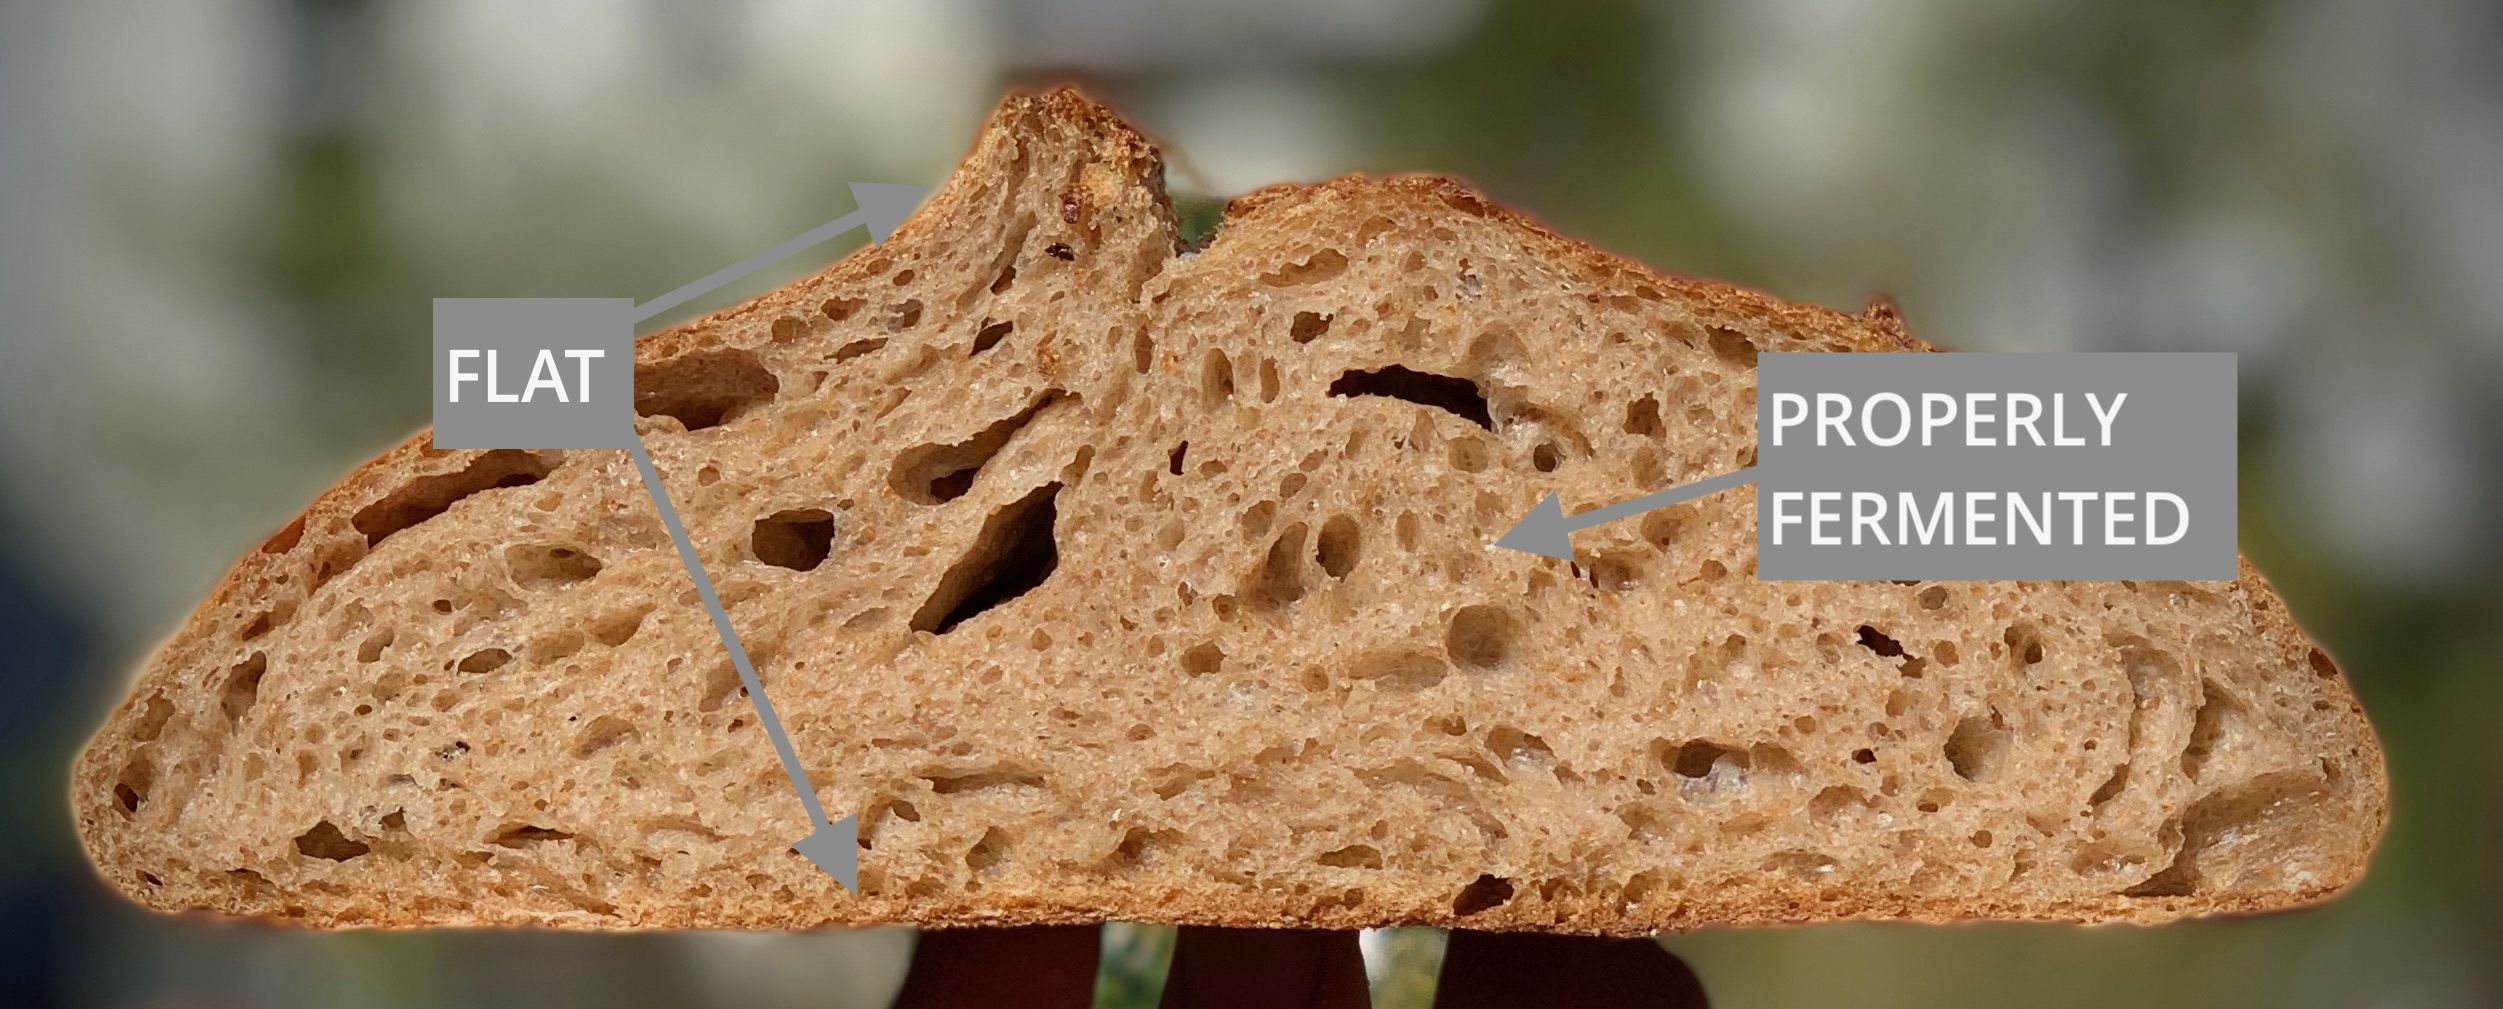
\includegraphics[width=\textwidth]{flat-bread}
  \caption{A very flat bread without enough dough strength.}%
  \label{flat-bread}
\end{figure}

When a dough flattens out quite a lot during the baking process, the chances are
that you did not create enough dough strength. This means your gluten matrix
hasn't been developed properly. Your dough is too extensible and flattens out
mostly rather than springing upwards in the oven. This can also happen if you
proofed your dough for too long. Over time the gluten relaxes and your dough
becomes more and more extensible. You can observe the gluten relaxing behavior
too when making a pizza pie. Directly after shaping your dough balls, it's very hard to shape
the pizza pie. If you wait for 30--90 minutes stretching the dough becomes a lot easier.

The easiest way to fix this is probably to knead your dough more at the start. To simplify
things consider using less water for your flour too. This will result in a more elastic dough
right away. This concept is commonly used for no-knead style sourdough.  Alternatively, you
can also perform more stretch and folds during the bulk fermentation process. Each
stretch and fold will help to strengthen the gluten matrix and make a more elastic dough.
The last option to fix a dough with too little dough strength is to shape your dough tighter.

\subsection{Baked too hot}

\begin{figure}
  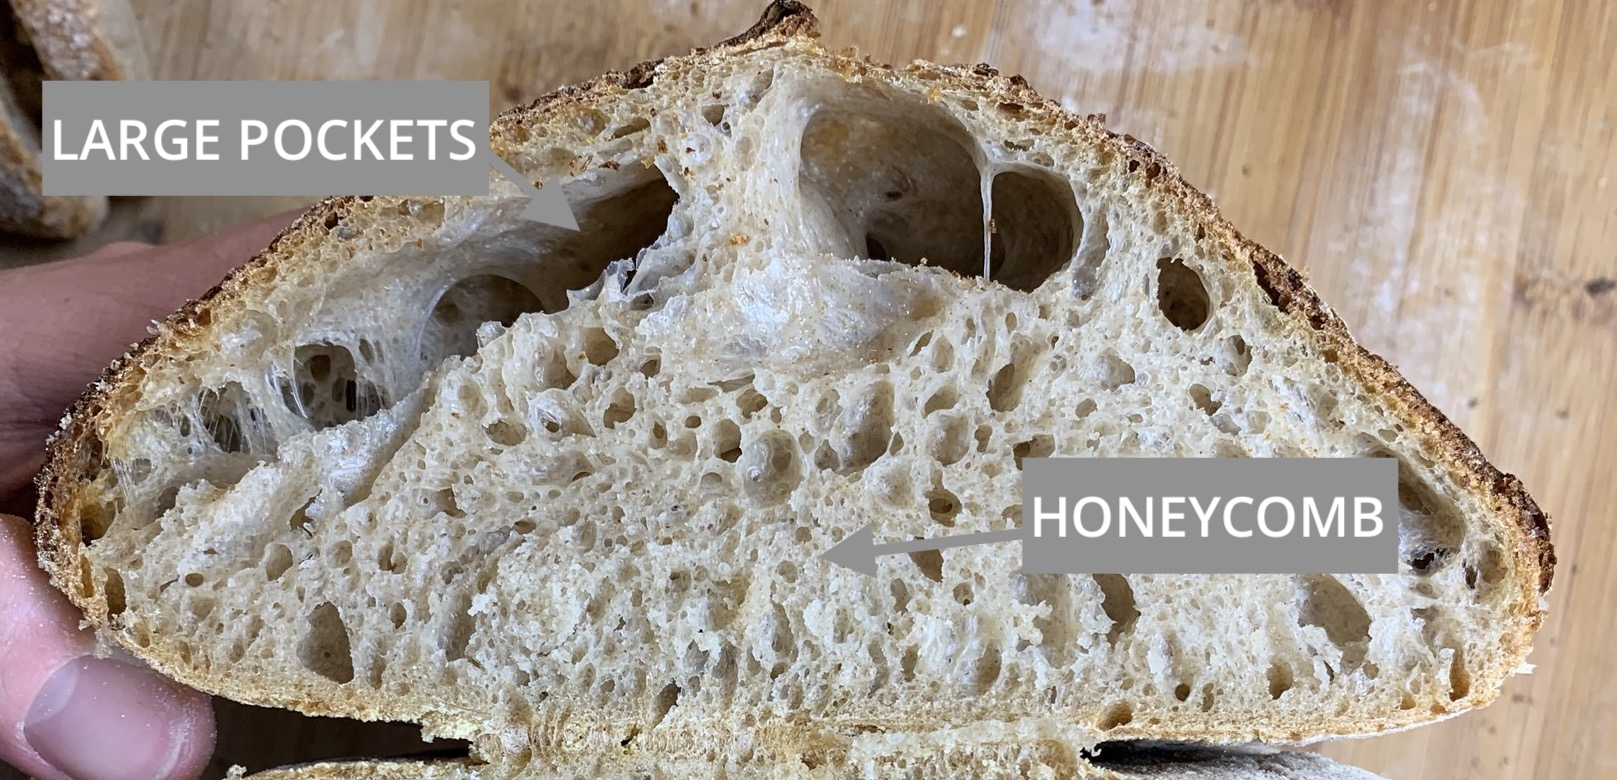
\includegraphics[width=\textwidth]{baked-too-hot-v2}
  \caption{A bread with very large alveoli close to the crust.}%
  \label{baked-too-hot}
\end{figure}

This is a common mistake that has happened to me a lot. When you bake your dough
at too high a temperature, you constrain your dough's expansion. The starch gelatinizes
and becomes more and more solid. At around 140°C (284°F) the Maillard reaction
starts to completely thicken your bread dough's crust. This is similar to baking
your bread dough without steam. As the internal dough's temperature heats up,
more and more water evaporates, gas expands and the dough is being pushed upwards.
Once the dough reaches the crust, it can no longer expand. The alveoli merge
into larger structures close to the surface of the dough. By baking too hot,
you are not achieving the ear which adds extra flavor. Furthermore, by restricting
it's expansion, the crumb will not be as fluffy as it could be.

If you have an extensible dough with high hydration, baking too cold will result
in the dough flattening out quite a lot. The gelatinization of the starch is
essential for the dough to hold its structure. After conducting several
experiments, it seems that my sweet spot for maximum oven spring seems to be
at around 230°C (446°F). Test the temperature of your oven, because in several
cases the displayed temperature might not match the actual temperature of your
oven~\cite{too+hot+baking}. Make sure to turn off the fan of your oven. Most
home ovens are designed to vent the steam as fast as possible. If you can not
turn the fan off, consider using a Dutch oven.

\subsection{Baked with too little steam}

\begin{figure}[h]
  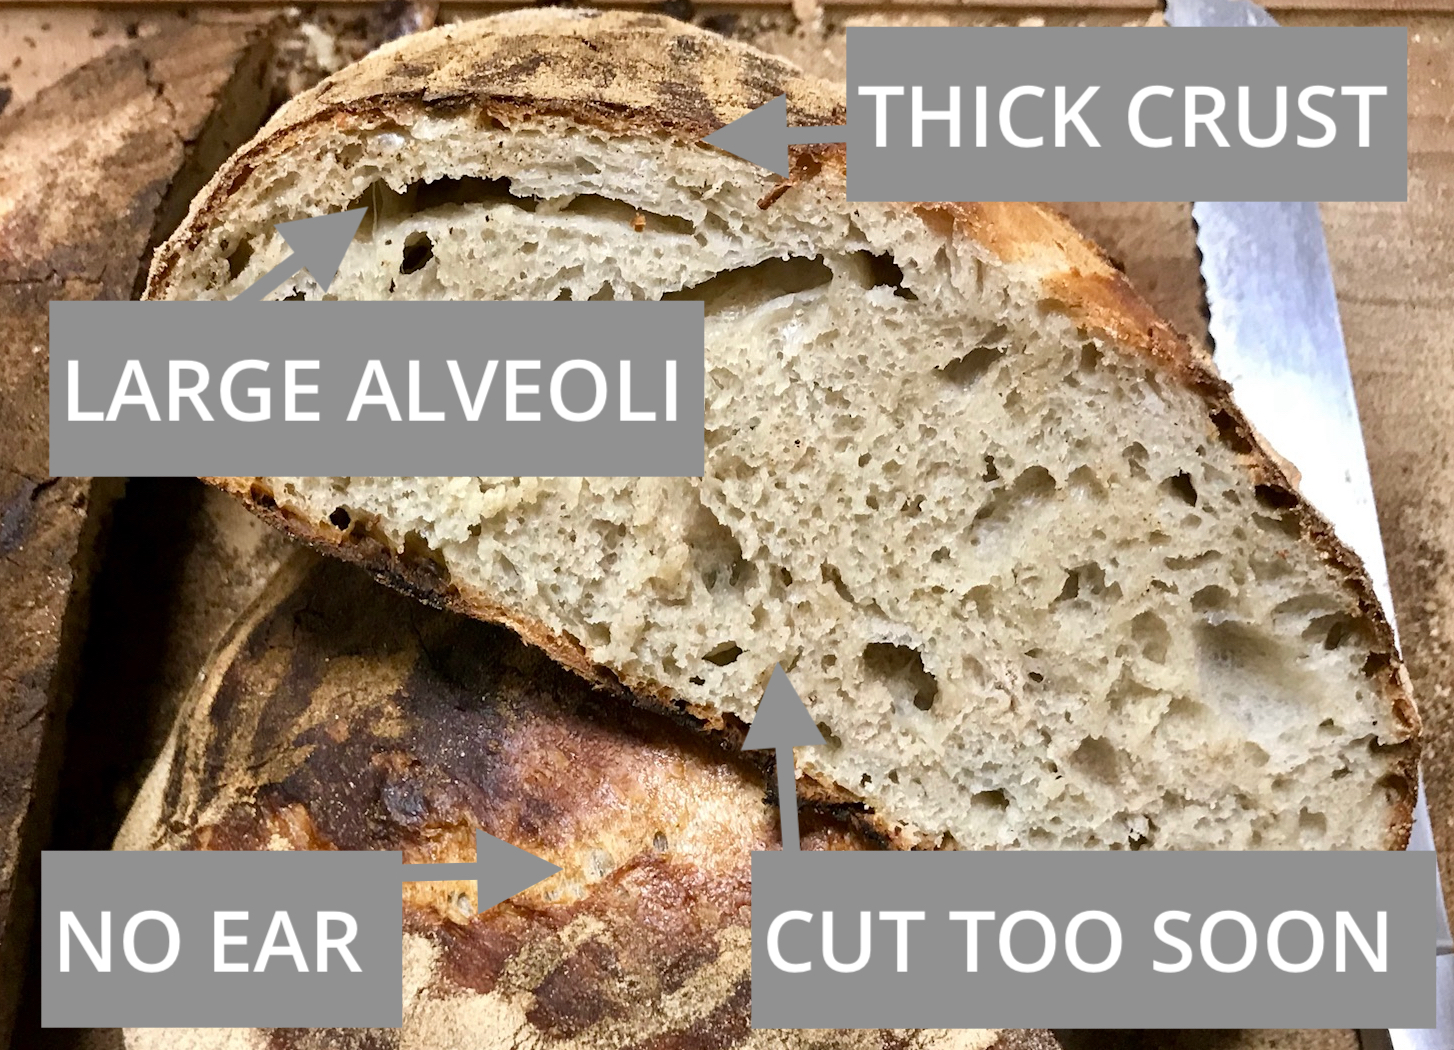
\includegraphics[width=\textwidth]{no-steam}
  \caption{One of my earlier breads that I~baked at a friend's place where
  I~couldn't steam the dough properly.}%
  \label{no-steam}
\end{figure}

Similar to baking too hot, when baking without enough steam, your dough's crust
forms too quickly. It's hard to spot the difference between the two mistakes.
I~typically first ask about the temperature and then about the steaming technique
to determine what might be wrong with the baking process. Too little steam can
typically be spotted by having a thick crust around all around your dough paired
with large alveoli towards the edges.

The steam essentially prevents the Maillard reaction from happening too quickly
on your crust. That's why steaming during the first stages of the bake is so important.
The steam keeps the temperature of your crust close to around 100°C (212°F). Achieving steam
can be done by using a Dutch oven, an inverted tray and/or a bowl of boiling water.
You might also have an oven with a built-in steam functionality. All the methods work,
it depends on what you have at hand. My default go-to method is an inverted
tray on top of my dough, paired with a bowl full of boiling water towards the bottom
of the oven.

\begin{figure}
  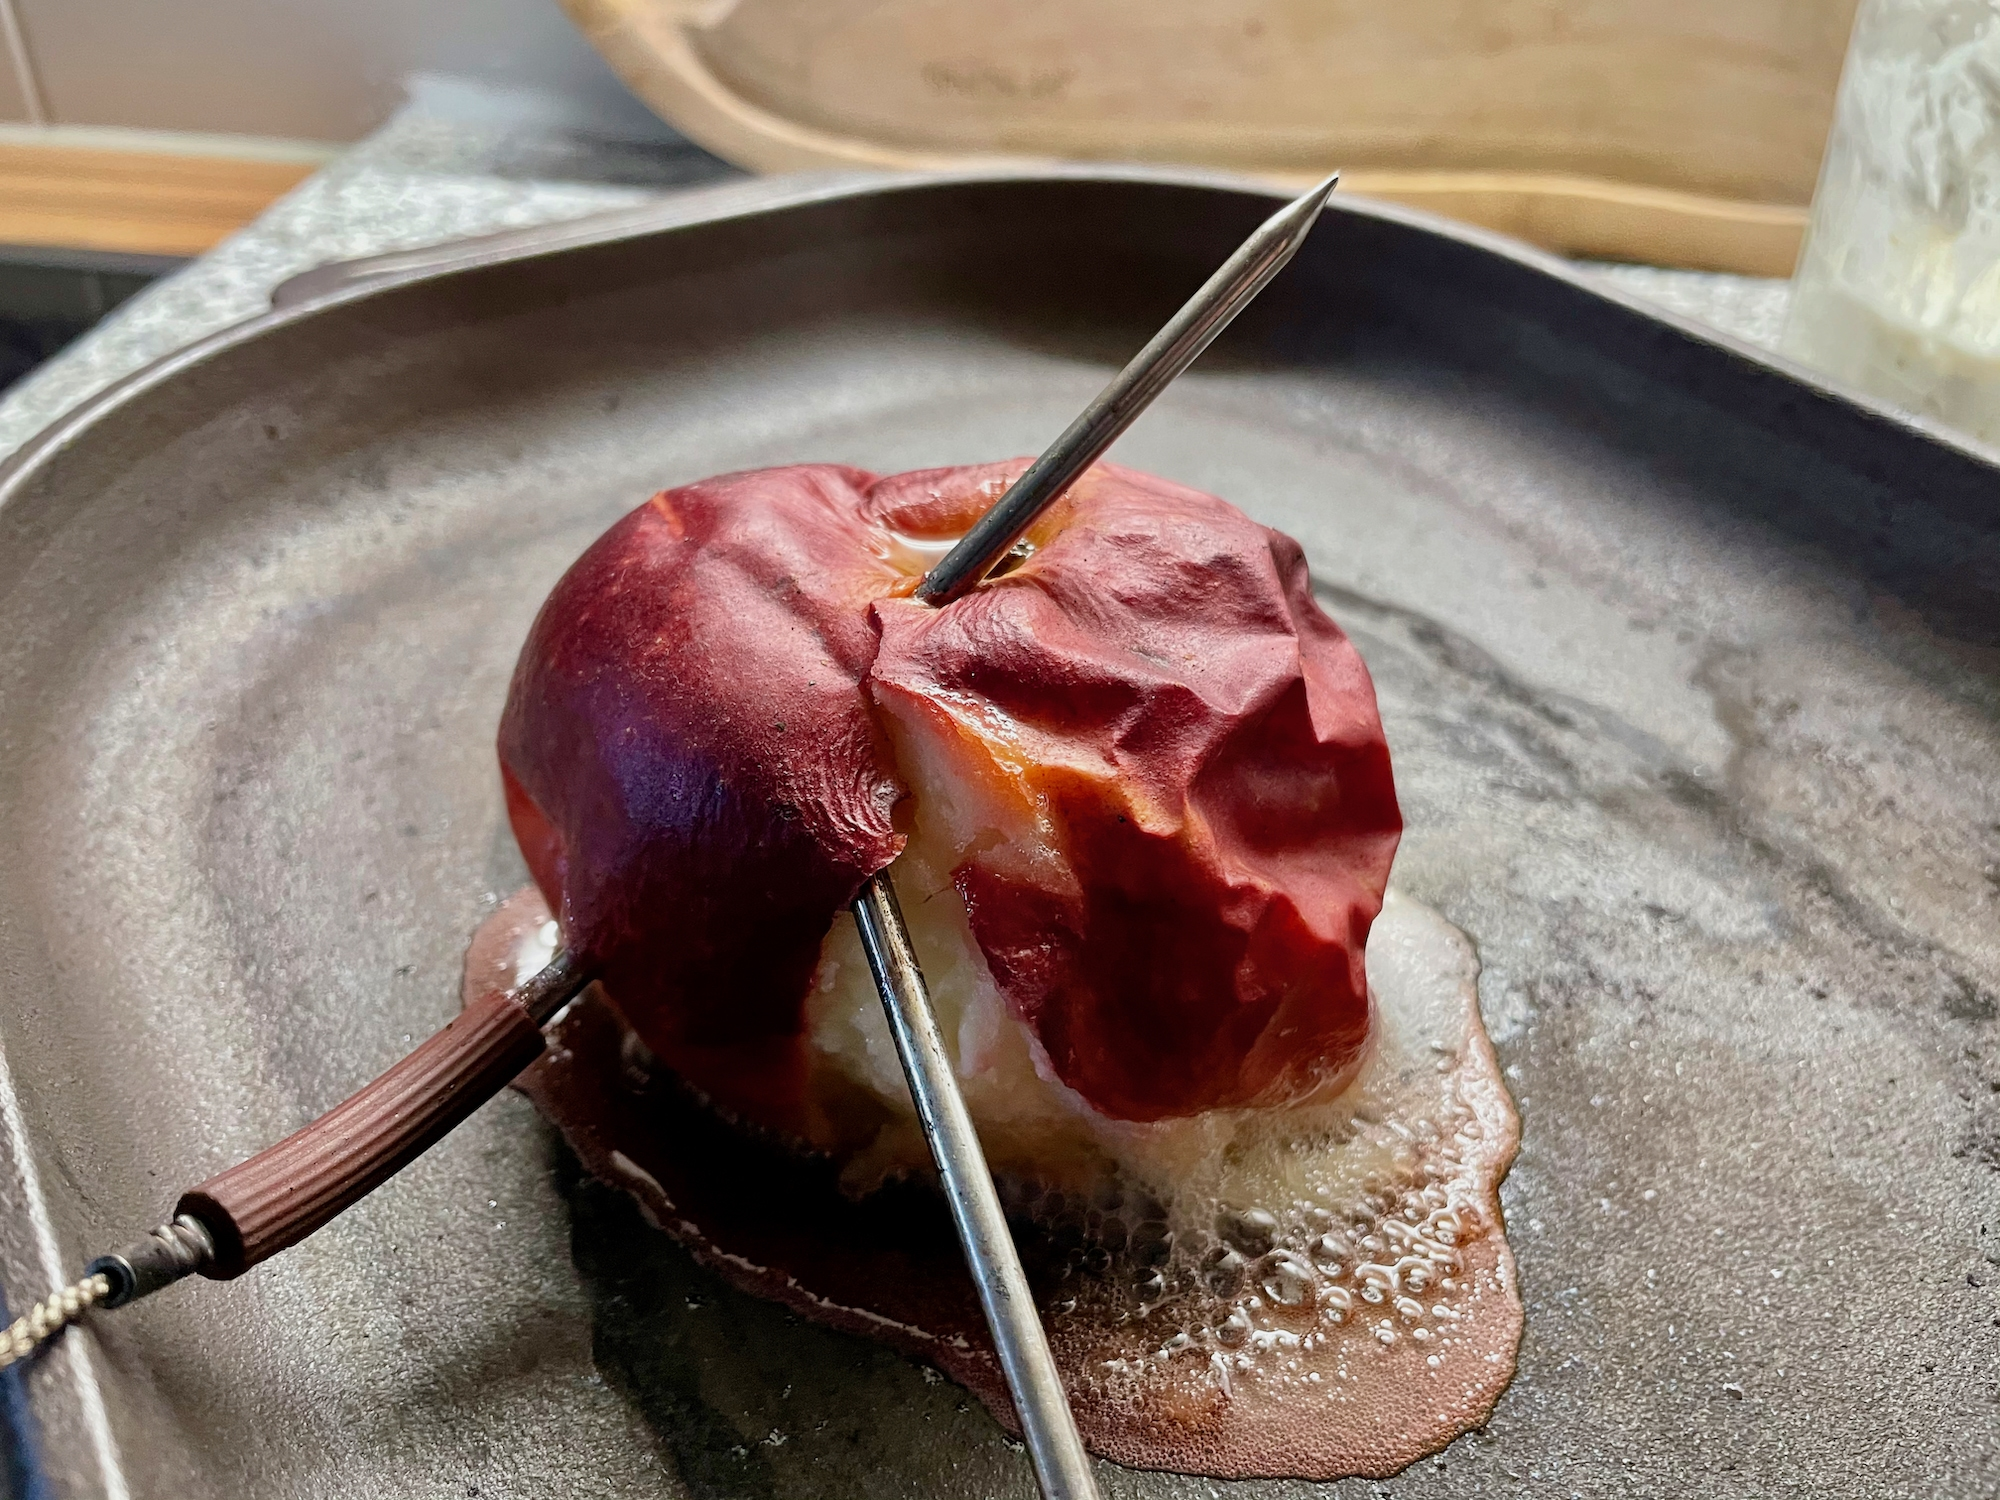
\includegraphics[width=\textwidth]{apple-experiment-temperatures}
  \caption{An apple with 2 probes to measure ambient
  and surface temperatures of several steaming techniques
  in a Dutch oven.}%
  \label{apple-experiment-temperatures}
\end{figure}

Now there can also be too much steam. For this I~tested using a Dutch oven paired with large ice
cubes to provide additional steam. The temperature of my dough's surface would directly
jump close to 100°C. The steam contains more energy and thus through convection
can heat up the surface of your dough faster. I~tested this by putting an apple inside
a Dutch oven and measuring its surface temperature using a barbecue thermometer.
I~then changed the steaming methods to plot how quickly the temperature
close to the surface changes. I~tested an ice cube inside of a preheated
Dutch oven, a preheated Dutch oven, a preheated Dutch oven with spritzes
of water on the apple's surface, a non-preheated Dutch oven where I~would only preheat
the bottom part. The experiment then showed that the ice-cube method would heat up
the surface of the apple a lot quicker. When replicating this with a bread dough,
I~would achieve less oven spring.

\begin{figure}[h]
  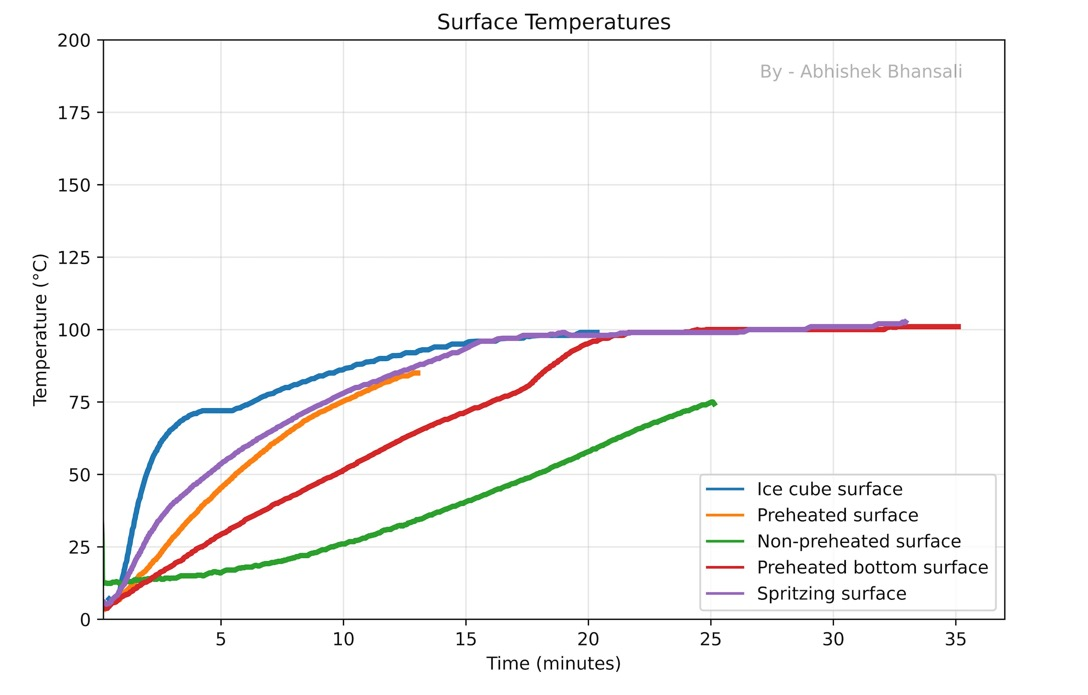
\includegraphics[width=\textwidth]{apple-experiment-surface-temperatures}
  \caption{A chart showing how the temperature of the surface
  of the apple changes with different steaming techniques.}%
  \label{apple-experiment-surface-temperatures}
\end{figure}

\begin{figure}[h]
  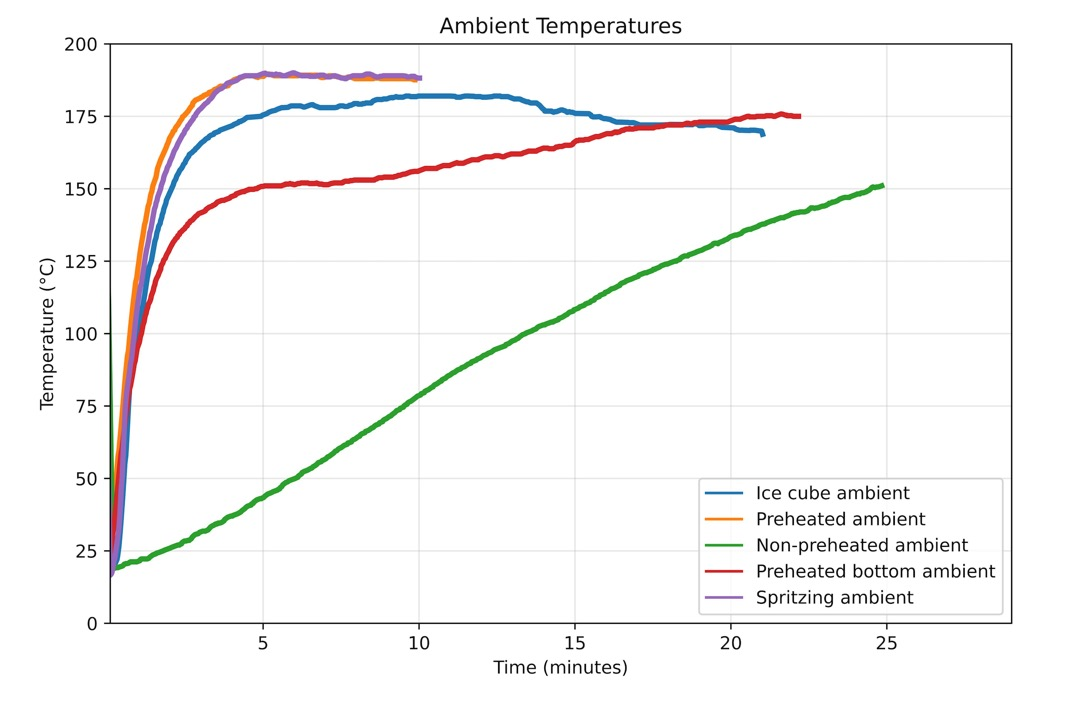
\includegraphics[width=\textwidth]{apple-experiment-ambient-temperatures}
  \caption{This figure shows how the ambient temperatures inside of the
  Dutch oven change depending on the steaming technique that is used.}%
  \label{apple-experiment-ambient-temperatures}
\end{figure}

Generally though, achieving too much steam is relatively challenging. I~could only
make this mistake when using a Dutch oven as the steaming method paired with relatively
large ice cubes. After talking with other bakers using the same Dutch oven, it seems
that my ice cubes (around 80g) were 4 times as heavy as the ones other bakers
would use (20g).


\section{Misc}
\subsection{Baking in the tropics}

Depending on the temperature, your fermentation speed adapts.
In a warmer environment, everything is faster. In a colder
environment, everything is slower.

This includes the speed at which your sourdough ferments
the dough but also the speed of enzymatic reactions. The
amylase and protease enzymes work faster, making more
sugars available and degrading the gluten proteins.

At around \qty{22}{\degreeCelsius} (\qty{72}{\degF}) in my kitchen my bulk fermentation is ready
after around 10~hours. I~use around \qty{20}{\percent} of sourdough
starter based on the flour. In summertime the temperatures
in my kitchen sometimes increase to
\qty{25}{\degreeCelsius} (\qty{77}{\degF}). In that case
I~reduce the sourdough starter to around \qty{10}{\percent}.

If I~didn't do that, my fermentation would be done after
around 4--7~hours. The problem is that the dough is quite
unstable when fermenting at this high speed. This means
that you easily run into issues of over-fermentation.
Finding the perfect sweet spot between fermenting enough
and not too much becomes much harder. Normally you might
have a time window of 1~hour. But at the rapid speed it
might be reduced to a time window of 20~minutes. Now at
\qty{30}{\degreeCelsius} (\qty{86}{\degF}), everything moves much faster. Your
bulk fermentation might be complete in 2--4~hours when using
\qtyrange{10}{20}{\percent} starter. Proofing your dough in the fridge becomes
almost impossible. As your dough cools down in the fridge the fermentation
also slows down. However cooling the dough down from \qty{30}{\degreeCelsius}
to \qtyrange{4}{6}{\degreeCelsius} in your fridge takes much longer. Your
dough is much more active compared to a dough that starts at a temperature of
\qtyrange{20}{25}{\degreeCelsius}. You might end up overproofing your dough if
you leave it overnight in the fridge.

That's why I~recommend that you reduce the amount of starter
that you use in the tropics to around \qtyrange{1}{5}{\percent}
based on the flour. This will slow down the fermentation
process significantly and provides you a bigger window
of time. Try to aim for an overall bulk fermentation of at
least 8--10~hours. Reduce the amount of starter to get there.

When making dough, try to use the same water temperature
as your ambient temperature. Assuming that the temperature
will climb to \qty{30}{\degreeCelsius} try to start your dough
with \qty{30}{\degreeCelsius} water. This means that you can carefully rely on
a small fermentation sample (aliquot jar) that visualizes your fermentation
progress. To read more about this technique refer
to Section~\ref{section:bulk-fermentation}.

The sample only works reliably if your dough temperature
is equal to your ambient temperature. Else the sample heats
up or cools down faster. So tread carefully when using
the sample in this case. It's always better to stop
the fermentation a little too early rather than too late.
Stretch and folds during the bulk fermentation
will help you to develop a better feel for
the dough. An expensive but possibly useful tool
could be a pH meter that allows you to perfectly
measure how much acidity has been created by the
lactic and acetic acid bacteria. In this case measure
the pH repeatedly and figure out a value that works
for your sourdough. In my case I~tend to end bulk
fermentation at a pH of around 4.1. Please don't just
follow my pH value; it's very individual. Keep measuring
with different doughs to find out a value that works for you.

\subsection{My flour has low gluten content --- what should I~do?}

You can always mix in a little bit of vital wheat gluten. Vital wheat gluten
is concentrated extracted gluten from wheat flour.

I~recommend that you add around \qty{5}{\gram} of wheat gluten for every
\qty{100}{\gram} of flour that you are using.

\subsection[Incorporating seeds into the dough]{What's the best stage to
incorporate inclusions (seeds) into the dough?}

You can include seeds directly at the start when mixing the dough. If you use
whole seeds such as wheat or rye kernels, soak them in water overnight and
then rinse them before adding them to the dough. This makes sure that they
are not crunchy and are soft enough when eating the bread. If you forgot to soak
them you can cook the seeds for 10~minutes in hot water. Rinse them with cold
water before adding them to your dough.

If you want to sweeten the dough, your best option is to add sugar during the
shaping stage. Sugar added too early in the process typically gets fermented until none of it
remains. Adjust your shaping technique a little bit and spread your sugar
mixture over a flattened-out dough. You can then roll the dough together,
incorporating layers of sugar.

